\documentclass[]{politex}

% ========== Opções ==========
% pnumromarab - Numeração de páginas usando algarismos romanos na parte pré-textual e arábicos na parte textual
% abnttoc - Forçar paginação no sumário conforme ABNT (inclui "p." na frente das páginas)
% normalnum - Numeração contínua de figuras e tabelas 
%	(caso contrário, a numeração é reiniciada a cada capítulo)
% draftprint - Ajusta as margens para impressão de rascunhos
%	(reduz a margem interna)
% twosideprint - Ajusta as margens para impressão frente e verso
% capsec - Forçar letras maiúsculas no título das seções
% espacosimples - Documento usando espaçamento simples
% espacoduplo - Documento usando espaçamento duplo
%	(o padrão é usar espaçamento 1.5)
% times - Tenta usar a fonte Times New Roman para o corpo do texto
% noindentfirst - Não indenta o primeiro parágrafo dos capítulos/seções


% ========== Packages ==========
\usepackage[utf8]{inputenc}
\usepackage{amsmath,amsthm,amsfonts,amssymb}
\usepackage{graphicx,cite,enumerate}
\usepackage{multirow}
\usepackage{todonotes}
\usepackage{csquotes}
\usepackage{listings}
\lstset{
  basicstyle=\ttfamily,
  columns=fullflexible,
  frame=single,
  breaklines=true,
  postbreak=\mbox{\textcolor{red}{$\hookrightarrow$}\space},
}
\usepackage{longtable}
\usepackage{rotating}
\usepackage{array}


% ========== Language options ==========
\usepackage[brazil]{babel}
%\usepackage[english]{babel}


% ========== ABNT (requer ABNTeX 2) ==========
%	http://www.ctan.org/tex-archive/macros/latex/contrib/abntex2
\usepackage[num, overcite]{abntex2cite}
\citebrackets{}

% Forçar o abntex2 a usar [ ] nas referências ao invés de ( )
%\citebrackets{[}{]}


% ========== Lorem ipsum ==========
\usepackage{blindtext}



% ========== Opções do documento ==========
% Título
\titulo{Moirai: sistema de detecção de uso de armas de fogo na borda computacional utilizando abordagem multicâmera}

% Para múltiplos autores (TCC)
\autor{Andrei Kenji Tsuda\\
		Felipe Caracciolo Gonçalves\\
		Rodrigo Dias Manduca}

% Orientador / Coorientador
\orientador{Prof. Dr. Marcelo Knörich Zuffo}

% Tipo de documento
\tcc{Eletricista com ênfase em Sistemas Eletrônicos}
%\teseDOC{Engenharia Elétrica}
%\teseLD
%\memorialLD

% Local
\local{São Paulo}

% Ano
\data{2019}




\begin{document}
% ========== Capa e folhas de rosto ==========
\capa
\falsafolhaderosto
\folhaderosto


% ========== Folha de assinaturas (opcional) ==========
%\begin{folhadeaprovacao}
%	\assinatura{Prof.\ X}
%	\assinatura{Prof.\ Y}
%	\assinatura{Prof.\ Z}
%\end{folhadeaprovacao}


% ========== Ficha catalográfica ==========
% Fazer solicitação no site:
%	http://www.poli.usp.br/en/bibliotecas/servicos/catalogacao-na-publicacao.html

% ========== Agradecimentos ==========
\begin{agradecimentos}

O grupo gostaria de agradecer ao Professor Marcelo Zuffo, por todo o apoio dado desde a concepção do projeto até sua execução, essencial para nosso sucesso, e pelas oportunidades concedidas.

\begin{center}
    \noindent\rule{2cm}{0.4pt}
\end{center}

Aos meus pais e minha irmã com quem pude contar em toda minha graduação, aos meus amigos que sempre me apoiaram e foram pacientes pela minha ausência durante minha dedicação ao projeto.

\begin{flushright}
	-{}- Andrei
\end{flushright}

A meus pais Ana e Antonio, e minha irmã Carolina pelo amor e apoio sempre. A minha família como um todo, por terem me proporcionado a oportunidade e o privilégio de uma educação de qualidade, sem o qual não estaria aqui. Ao cachorro Thor pelo amor incondicional, todos os dias.

A meus amigos Cocóusados, Maria Júlia, Isabella, Thomas, Gabriela e Bruno, parceiros de mais de 15 anos, pelos momentos compartilhados e por estarem sempre por perto, de uma forma ou de outra.

Ao Guigo, pela parceria e companhia quase que inseparável nesses últimos anos. Aos amigos do Full, pela amizade e pela companhia intensas, ainda que mais recentes: vocês também são fruto da minha passagem pela Poli.

À univerisdade pública, por, mesmo com suas limitações e estando sob ataque, continuar existindo e proporcionando oportunidades: que elas possam se estender a todos os cidadãos que a elas têm direito.

\begin{flushright}
	-{}- Felipe
\end{flushright}
	
A meus pais e minhas irmãs, por me não me deixarem desistir, por me fazerem enxergar mais claramente o futuro e por estarem comigo em todos os momentos. Amo vocês.

Ao meu Vô João, que foi minha inspiração máxima na vida. Obrigado pelas viagens, ensinamentos, almoços estranhos e leilões do Mr. Fumaça. Esse diploma é pra você.

Aos meus FULL amigos otários, por acreditarem em mim, mesmo quando eu mesmo já não acreditava e por tornar estes últimos 6 anos os melhores da minha vida.

Um agradecimento especial ao meu querido amigo Snowden, companheiro de todas as festas, amigo pra (quase) todas as horas e parceiro de todos os trabalhos. Na Poli, não há um Guigo sem Snow e nem um Snow sem Guigo. TAN!

\begin{flushright}
	-{}- Rodrigo
\end{flushright}
\end{agradecimentos}


% ========== Epígrafe (opcional) ==========
 \epigrafe{
 
\emph{``A experiência mais bonita que podemos ter é o mistério. É a emoção fundamental que está no berço da verdadeira arte e da verdadeira ciência. Quem não sabe disso e não consegue mais se maravilhar poderia tão bem estar morto.''}
\begin{flushright}
	-{}- Albert Einstein
\end{flushright}

\vspace{4.5\baselineskip}

\emph{``I rock, I roll, I bloom, I grow''}
\begin{flushright}
	-{}- Tyler Okonma
\end{flushright}

\vspace{4.5\baselineskip}

\emph{``Well, here at last, dear friends, on the shores of the sea comes the end of our fellowship in middle-earth. Go in peace! I will not say: do not weep for not all tears are an evil.''}
\begin{flushright}
	-{}- Gandalf
\end{flushright}
}

% ========== Resumo ==========
\begin{resumo}
A escalada de violência armada no Brasil vem se intensificando nos últimos anos, criando a necessidade de novas abordagens para a segurança pública. Sendo assim, o objetivo do trabalho é desenvolver um algoritmo de visão computacional que permita a detecção de armas de fogo, gerando alertas automáticos que seriam encaminhados autoridades de segurança competentes. Considerando-se a natureza distribuída que o monitoramento de uma grande cidade exige, as especificações técnicas desse algoritmo baseiam-se na execução em computação de borda, com requisitos de software e consumo de energia condizentes com esse paradigma. No entanto, essa mudança de paradigma exige que algumas concessões de precisão e velocidade sejam feitas. È proposta então, uma arquitetura de câmeras múltiplas, agregadas por um classificador linear que procura compensar as concessões realizadas para a construção de um modelo viável.
%
\\[3\baselineskip]
%
\textbf{Palavras-Chave} -- Computação de borda, Detecção de imagens, Segurança pública, Ensemble learning, Redes neurais, YOLO.
\end{resumo}

% ========== Abstract ==========
\begin{abstract}
Gun violence in Brazil is on the rise, raising the need for new public security approaches. The goal of this work is to develop a computer vision algorithm capable of detecting handgun use, generating automatic alerts to be sent to the competent authorities. Considering the distributed nature required by a big city's monitoring system, this algorithm's technical specifications are based on edge computing execution, presenting matching software and energy consumption capabilities. On the other hand, this paradigm shift means compromises are made to precision and speed metrics. A multiple camera architecture is then proposed, aggregating predictions using a linear classifier in an attempt to create a more feasible model.
%
\\[3\baselineskip]
%
\textbf{Keywords} -- Edge computing, Image detection, Public security, Ensemble learning, Neural networks, YOLO.
\end{abstract}

% ========== Listas (opcional) ==========
\listadetabelas
\listadefiguras

% ========== Sumário ==========
\sumario



% ========== Elementos textuais ==========

\chapter{Introdução}

Nesse trabalho, iremos analisar a viabilidade, por meio da implementação e teste, de um algoritmo de visão computacional de detecção de armas aplicado em uma infraestrutura distribuída, ou seja, na borda computacional. Esse algoritmo deve ser capaz de identificar o uso de armas de fogo e alertar as autoridades competentes.

Trabalhos anteriores\cite{olmos1} já foram desenvolvidos aplicando a prática de \textit{transfer learning} a algoritmos de detecção de imagem existentes para aplicação em tempo real para armas de fogo. Após estabelecida as motivações, e esclarecidos os fatores envolvidos, contextualizaremos esse trabalho e o problema de forma geral em um novo escopo: a utilização em sistemas embarcados distribuídos de baixo custo.

Para tal, analisaremos os fatores positivos e negativos relacionados a cada algoritmo, arquitetura e escolha de projeto. Em seguida, faremos uma aplicação prática da solução desenvolvida e analisaremos seu potencial e viabilidade.

\section{Motivação}

Na manhã do dia 13 de março de 2019, dois adolescentes entraram na escola estadual Raul Brasil em Suzano, São Paulo, e, armados de uma pistola e uma besta, atiraram contra alunos, professores e funcionários da escola. O ataque deixou 10 mortos e 11 feridos, tornando-se um dos mais chocantes massacres da história do estado de São Paulo, reacendendo o debate sobre o porte de armas de fogo no país.

Segundo informações da polícia\cite{noticiapolicia}, foram realizadas 69 ligações vindas de pessoas que escutavam o tiroteio de suas casas, que passavam pelo local e observando a correria ou até de alunos que conseguiram se esconder nas salas da escola. A primeira ligação aconteceu passado um período relativamente longo do começo do ataque, e ainda assim as informações passadas à Polícia Militar e ao Corpo de Bombeiros eram difusas e não aderiam bem aos fatos, resultado de um reflexo natural do processo de compreensão dos acontecimentos e expressão dos mesmos por parte de seres humanos quando envolvidos em situações emergenciais. No entanto, a demora e as inconsistências, bem como o subsequente pico na carga dos sistemas de atendimento emergencial locais fizeram com que o tempo de resposta para o caso fosse maior do que o ideal.

Durante as investigações sobre o caso, as imagens das câmeras de segurança atuaram como elemento central no entendimento do ocorrido e na identificação dos culpados, mostrando em detalhes a utilização das armas de fogo pelos atiradores. Apesar das câmeras em questão serem de circuito fechado, surge a reflexão: se as câmeras foram capazes de gravar o crime e apontar os responsáveis, por que as mesmas não poderiam ser utilizadas em sua prevenção, ou, ao menos, no desenrolar do tiroteio? Poderiam essas mesmas câmeras ajudar no acionamento da Polícia Militar e do Corpo de Bombeiros, mitigando a falha humana ao relatar emergências?

O Atlas da Violência 2019\cite{atlasdaviolencia} publicado pelo Instituto de Pesquisa Econômica Aplicada, vinculado ao Governo Federal, aponta que, apesar de se observar uma tendência à diminuição do número absoluto de homicídios na maioria das unidades federativas do Brasil, quando se trata de homicídios causados por armas de fogo, a maioria dos estados apresenta um aumento no número de casos, seja em valores absolutos, relativo à taxa por 100 mil habitantes.

No entanto, um fator importante que se destaca no relatório é a discrepância entre as métricas de certas unidades federativas. Em São Paulo, estado que comprovadamente investiu em políticas públicas centradas na retirada de armas de fogo de circulação, se apresentou uma diminuição em todas as métricas anteriormente citadas sobre homicídios por armas de fogo, enquanto no Acre, estado que não contou com as mesmas políticas e ainda sofreu com forte atuação de facções criminosas, o aumento nas mesmas foi monstruoso.

\begin{table}[ht]
\centering
\begin{tabular}{lcccl}
\cline{1-4}
\multicolumn{4}{c}{\textit{\textbf{Variação (de 2007 a 2017)}}}                                                                                                  &  \\ \cline{1-4}
\multicolumn{1}{|l|}{\textbf{UF}}        & \multicolumn{1}{l|}{\textbf{Absoluto}} & \multicolumn{1}{l|}{\textbf{Taxa}} & \multicolumn{1}{l|}{\textbf{Proporção}} &  \\ \cline{1-4}
\multicolumn{1}{|l|}{\textit{São Paulo}} & \multicolumn{1}{c|}{-39,3\%}           & \multicolumn{1}{c|}{-43,9\%}       & \multicolumn{1}{c|}{-18,0\%}            &  \\ \cline{1-4}
\multicolumn{1}{|l|}{\textit{Acre}}      & \multicolumn{1}{c|}{652,9\%}           & \multicolumn{1}{c|}{538,4\%}       & \multicolumn{1}{c|}{97,0\%}             &  \\ \cline{1-4}
\end{tabular}
\caption{Dados do Atlas da Violência acerca da variação, no período de 2007 a 2017, no valor absoluto de homicídios, na taxa por 100 mil habitantes e na proporção em relação a a todos os homicídios nos estados de São Paulo e Acre}
\label{tbl:atlasdaviolencia}
\end{table}

Evidenciando as causas e consequências de dados como os apresentados na tabela \ref{tbl:atlasdaviolencia}, o relatório é concluído com um apelo por políticas de segurança pública que não só ataquem a raíz do problema (a desigualdade social gritante no Brasil), mas que também procurem contrapor a flexibilização do uso e porte de armas de fogo que está em curso no país (e que é comprovadamente prejudicial), e que foquem em inteligência policial e investigação.

Dado isso, uma solução tecnológica focada na detecção de armas e uma subsequente tentativa de prevenção de seu uso parece estar alinhada com as melhores práticas de segurança pública, apresentando benefícios para além da óbvia proteção às potenciais vítimas de violência armada. Um sistema com essa capacidade permite, por sua natureza, que também seja feito um amplo levantamento de dados e estatísticas, além, é claro, da utilização de imagens para o esclarecimento do desenrolar dos casos. Ou seja, tal sistema ajudaria tanto na inibição do uso de armas de fogo quanto na construção de uma inteligência policial mais robusta.

Conforme veremos nas próximas seções, outros aspectos do projeto serão decididos com base em fatores que influenciam a aplicação do sistema em uma esfera prática e pública, como escalabilidade, distributividade, custo, governança e outros.

\section{O estado da IA e a borda computacional}

Não é surpreendente que, seguindo a tendência dos últimos anos, o volume de dados trafegado na internet esteja em um processo de aumento exponencial. Tal crescimento pode ser atribuído a diversos fatores, desde a democratização do acesso à Internet e da redução de custo de smartphones, até a expansão da Internet das Coisas e a popularização do \textit{streaming} de vídeo. A largura de banda começa, então, a se tornar um gargalo para a viabilidade de sistemas inteligentes mais avançados, criando a necessidade para tecnologias de telecomunicações como o 5G, que encontra-se em fase de implementação, mas ainda levará muitos anos para estar amplamente disponível. Concomitantemente, o avanço tecnológico em pesquisas de hardware faz com que tenhamos acesso a um poder computacional cada vez maior no estado da arte e, seguindo diretamente essa tendência, hardware menos avançado, porém extremamente miniaturizado e a um custo baixo. Esses movimentos são a base para o surgimento de conceitos como o de \textit{Mobile Edge Computing}, descrito em \citeyear{mectaxonomy} \citeauthor{mectaxonomy}, e o de \textit{Fog Computing} em \citeyear{fogcomputing} \citeauthor{fogcomputing}.

De acordo com o mais recente relatório do Cisco Visual Networking Index\cite{cisco}, conexões M2M (\textit{machine-to-machine}), referentes a dispositivos da Internet das Coisas, serão as que mais crescerão no período entre 2017 e 2022, com uma taxa de crescimento anual composta de 19\%. Ao final do período, serão 14.6 bilhões de dispositivos conectados, representando 51\% do total de dispositivos. Outra tendência interessante apresentada pelo relatório se refere à vídeo de câmeras de segurança na nuvem: em 2022, a simples transmissão (sem nenhuma análise sendo feita em cima do material) desse tipo de dado corresponderá a 3\% de todo o tráfego de vídeo na Internet.

Apesar do prognóstico otimista, é importante lembrar o contexto em que estamos inseridos. O Cisco Virtual Networking Index aponta que o volume de dados trafegados vindos da América Latina terá uma taxa de crescimento anual composta de 21\%, chegando a 19 exabytes por mês em 2022. No entanto, isso ainda representará 4,7\% do volume de tráfego mundial. No Brasil, a implementação da rede 5G deve ocorrer apenas em 2021, levando ainda mais tempo para se difundir e popularizar.

Para a implementação de um sistema de detecção de imagens, portanto, devemos levar em consideração as limitações impostas pelo fato do Brasil ser um país em desenvolvimento. Por outro lado, os algoritmos de detecção mais avançados se baseiam em \textit{deep learning}, ou seja, exigem, no mínimo, longos periodos de treinamento em hardware computacionalmente poderoso. Os conceitos de Fog e Edge computing propõem arquiteturas híbridas, onde o processamento de dados é feito em camadas mais próximas àquela onde são coletados os dados, se aproveitando do poder computacional (menos intenso) disponível ao longo da infraestrutura e removendo a necessidade de que todo trabalho feito em cima dos dados seja realizado em um grande servidor central enquanto o resto da rede tenha apenas a função de transporte.

No caso presente, essas topologias parecem se adequar às necessidades e condições existentes. Suponhamos um conjunto distribuído de câmeras de segurança que alimentasse um detector de armas de fogo único e centralizado. Uma infraestrutura como essa ainda exigiria certo nível de inteligência acoplada às câmeras, para que essas se comunicassem com o servidor central, fazendo o \textit{streaming} de vídeo de forma correta e segura. Além disso, seria necessária uma rede com banda e velocidade suficiente para receber os dados, que tem tamanho grande, bem como um servidor central com capacidade para suportar a carga de diversas câmeras se conectando a ele ao mesmo tempo.

\begin{figure}[ht]
  \centering
  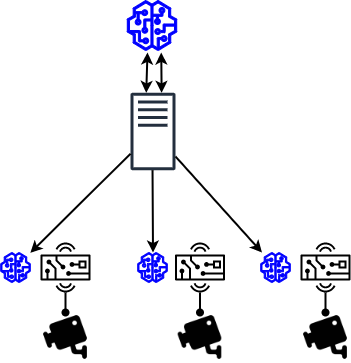
\includegraphics[scale=0.7]{img/diagrama.png}
  \caption{Diagrama demonstrando, de maneira simplificada, uma arquitetura híbrida de edge computing para o problema}
  \label{fig:diagramaarquitetura}
\end{figure}

No entanto, se organizarmos nosso sistema como o diagrama da figura \ref{fig:diagramaarquitetura} mostra, estaríamos reunindo conceitos de \textit{edge computing} a processamento em nuvem, promovendo um equilíbrio entre as arquiteturas. Como o treinamento de um sistema de detecção de imagem exige hardware poderoso e leva tempo, o mesmo seria realizado em uma unidade central mais poderosa, que contaria como recursos como grande quantidade de memória e aceleração por GPU. No entanto, nessa topologia, o modelo já treinado seria distribuído a \textit{single-board computers} acoplados às câmeras de segurança, que seriam responsáveis por executar a detecção em si, desonerando assim a rede entre essas duas camadas do transporte de gigabytes de dados de vídeo.

Tal topologia funciona especialmente nesse caso pois, em se tratando de câmeras de segurança, a relevância das imagens está estritamente limitada à área geográfica na qual a mesma está posicionada, . Podendo a detecção ser feita \textit{in-loco}, não há uma perda significativa de informação valiosa, pois as autoridades também podem ser acionadas de forma remota a partir do resultado da detecção. Além disso, podemos desenvolver a arquitetura apresentada na figura \ref{fig:diagramaarquitetura} para levar em consideração a geração de metadados e inferências que podem ser extraídos, localmente, da análise das imagens das câmeras, resultando em uma redução de dimensionalidade dos dados que viabiliza o seu transporte. Poderia ser implementado, inclusive, um fluxo de realimentação, onde imagens das câmeras de segurança fossem passadas ao servidor central para que passem a constituir o \textit{dataset} de treinamento do modelo, buscando melhorar sua precisão.

Parece adequado, portanto, que a solução proposta se valha de uma arquitetura semelhante. Contudo, o modelo aqui proposto está delineado de maneira ampla e em alto nível. A opção por um sistema que utilize \textit{edge computing} não virá sem seus \textit{trade-offs}, especialmente no que se refere à diferença de capacidade de hardware entre seus diversos componentes.

Dificilmente uma espécie de servidor central como o demonstrado na arquitetura simplificada esbarrará em barreiras técnicas ao longo da execução da proposta. No entanto, apesar do estado avançado dos \textit{single-board computers} e de sistemas embarcados, é possível que as capacidades de hardware e software da camada de borda ainda não apresentam um desempenho tão satisfatório quanto o de um hardware mais consolidado. No entanto, como o verdadeiro gargalo encontra-se em fatores mais críticos a realização do projeto, como fatores de custo ou até limitações de viabilidade real do projeto (que no caso da largura de banda para transmissão de dados pode até ser considerada uma limitação física), optamos por atacar esses pontos e então contornar limitações de hardware que possam surgir, possivelmente a algum custo mas garantindo o funcionamento do projeto de qualquer forma.

\section{Hardware, software e governança}

Estabelecida uma motivação, uma proposta de solução e uma ideia geral de arquitetura, devemos avançar para a definição de aspectos mais concretos e práticos da execução do projeto. Devemos, portanto, optar por componentes de software e hardware que comportem as especificações desejadas. No entanto, inicialmente damos um passo pra trás e analisamos outros aspectos externos à solução puramente tecnológica, mas que perpassam e contextualizam a solução, como transparência, governança e custo.

Primeiramente, devemos reconhecer as implicações da existência de uma ampla rede de vigilância no direito à privacidade das pessoas. Segundo \citeyear{firmino} \citeauthor{firmino}, a implementação de uma ampla rede de vigilância por meio de câmeras de segurança constitui uma nova camada de territorialização que se sobrepõe às já existentes camadas físicas, que influenciam o acesso e a circulação das pessoas que ocupam os espaços vigiados. Ou seja, ao transitar por um lugar, o indivíduo não só está condicionado às possibilidades físicas apresentadas pelo espaço (como barreiras de acesso, dificuldades de locomoção, etc.), mas também passa a poder sofrer ação como consequência da sua presença nas imagens das câmeras de segurança. As regras que regem essas potenciais ações não ficam claras, e muitas vezes não são decididas democraticamente, como em casos em que câmeras de segurança geridas de maneira privada estão apontadas para espaços públicos (como uma câmera de uma residência voltada para a rua, por exemplo). No caso do projeto aqui apresentado, cuja função é acionar as autoridades competentes de maneira automática, esse fator é ainda mais agravado, pois as consequências na vida dos sujeitos impactados podem ser devastadoras.

Levantamos assim a importância de que se traga uma garantia maior da manutenção da privacidade das pessoas que estarão circulando nos espaços públicos monitorados e que estarão submetidas a análise do algoritmo. Ao ocuparem esse lugar, é apenas seu direito que tenham uma boa visibilidade de como elas e suas ações serão analisadas e classificadas, visto que a utilização de uma solução automatizada, ainda que em teoria possa remover viéses causados pela avaliação humana, ainda é sujeita a falhas. 

Em \citeyear{dio} \citeauthor{dio} essa preocupação é levantada, sob o argumento de que a transparência sobre aparatos de vigilância é um ponto de partida para que a sociedade, de forma conjunta, debata o papel dessas tecnologias no cotidiano e, mais do que isso, possam impedir que esses aparatos sejam fontes de repressão e abusos, garantindo que exerçam sua função de maneira justa e responsável. A proposta estabelecida no artigo é a criação de um videogame que possui o objetivo de mapear a presença de câmeras de segurança por meio de \textit{crowdsourcing}, mas considerando que no trabalho presente estamos criando um novo sistema de segurança desde sua concepção, existem outras medidas que podem ser incorporadas diretamente ao projeto e que possam reforçar esses valores. A primeira, e que está fora do escopo desse trabalho, é o estabelecimento de uma Política de Privacidade e de mecanismos de asseguramento de uma governança correta e democrática desse sistema. Em segundo lugar, temos a adoção, na medida possível, dos paradigmas de software e hardware abertos nesse projeto.

Ao abrir ao público a composição do hardware e do software utilizados, mitigamos, de certa forma as preocupações em relação a transparência. Mas, para além disso, o uso de paradigmas abertos também representa uma maior segurança e confiabilidade no funcionamento do algoritmo e dos seus sistemas acoplados. Ainda que possa parecer contraintuitivo em um primeiro momento, pois revelar o código-fonte e o projeto de hardware possa ser um chamariz para atuações criminosas, o benefício que se obtém e que supera em muito os aspectos negativos é o engajamento de todo o resto da sociedade em uma comunidade centrada na identificação de falhas e bugs, no refinamento e desenvolvimento e do exercício de governança. 

Estabelecidos esses paradigmas, uma escolha natural para ser o hardware base do sistema proposto é a placa Labrador, do programa Caninos Loucos, responsável pelo desenvolvimento de soluções de hardware e software livre para Internet das Coisas. Segundo a documentação da Caninos Loucos Labrador\cite{doccaninos}:

\begin{quote}
A placa Labrador é a primeira Single Board Computer da Caninos Loucos, aberta e com as funcionalidades de um computador. É capaz de rodar em um sistema operacional Android ou Linux, acessar a internet por cabo de rede ou Wi-Fi, reproduzir vídeos e executar programas de edição de texto.

A Labrador é uma combinação de 2 placas, a core board, uma placa de tamanho reduzido e alta capacidade de processamento, e a base board, onde encontramos as diversas interfaces de comunicação.
\end{quote}

Além da estrutura aberta, a Caninos Loucos já tem sua utilização prevista em projetos futuros relacionados ao poder público na cidade de São Paulo. Ao analisarmos suas especificações técnicas, presentes na tabela \ref{tbl:specs}, também observamos que o hardware apresenta robustez suficiente para ser considerado como o objeto de estudo desse trabalho.

\begin{table}[ht]
\centering
\begin{tabular}{|l|l|}
\hline
\multicolumn{2}{|c|}{\textbf{Core Board (V2.0)}} \\ \hline
\multirow{2}{*}{CPU} & Quad-core ARM® Cortex™ 1,3GHz \\ \cline{2-2} 
 & A9R4 CPU (ARM v7 instruction set) \\ \hline
GPU & Imagination PowerVR SGX544 \\ \hline
\multirow{2}{*}{Memória} & 2 GB DDR3 SDRAM \\ \cline{2-2} 
 & 16GB eMMC \\ \hline
\multirow{2}{*}{Sistemas Operacionais} & Android 5.0 \\ \cline{2-2} 
 & Linux 3.10.100 \\ \hline
\multicolumn{2}{|c|}{\textbf{Base Board M (V1.0)}} \\ \hline
Armazenamento & MicroSD Card Slot SD/SDHC/SDXC (até 32GB) \\ \hline
\multirow{2}{*}{Câmera} & MIPI-CSI1 \\ \cline{2-2} 
 & Interface paralela de 8-bits \\ \hline
Alimentação & 5$\sim$12V@2A \\ \hline
\end{tabular}
\caption{Especificações técnicas da Caninos Loucos Labrador}
\label{tbl:specs}
\end{table}

Ao aplicarmos algoritmos de detecção, nos basearemos fortemente no estado da arte atual, que consiste em algoritmos desenvolvidos academicamente e que comprovadamente representam os melhores e mais rápidos métodos. Por serem trabalhos publicados, muitos desses algoritmos também possuem implementações em código aberto, das quais nos aproveitaremos. Sendo assim, e dados os motivos previamente apresentados, faz sentido que a solução desenvolvida também seja publicada como código aberto, sob uma licença MIT, que prevê uso, cópia, modificação, mesclagem, publicação, distribuição e venda de copias do software gratuitamente, no entanto isentando os autores de garantias e responsabilidades. É importante notar que, enquanto para o escopo aqui contemplado essas atribuições possam fazer sentido, em uma aplicação efetivamente prática do projeto, algumas partes do código e detalhes de implementação podem ser omitidas por questões de segurança da informação e de comunicações.

\section{Escopo e domínio de trabalho}

Estabelecida a parte introdutória e para que tenhamos um escopo bem delineado e adequado às proporções de um trabalho do formatura, vamos, finalmente estabelecer os parâmetros e as premissas que nortearão o desenvolvimento do trabalho.

A ideia é caminhar em direção a elaboração de um sistema completamente produtizado, porém de código aberto, de detecção de uso de armas de fogo com a capacidade de acionar automaticamente as autoridades, que seja facilmente escalável e distribuível, seguindo uma arquitetura de \textit{edge computing} e que tenha baixo preço. Futuramente, esse sistema também poderá ser modificado para coleta de dados e insights, bem como identificação de outros tipos de ocorrências.

No entanto, nesse trabalho focaremos no desenvolvimento do algoritmo de detecção em si, e na sua performance sob diferentes aspectos e sendo executado numa arquitetura de \textit{edge computing}, avaliando as limitações já mencionadas na seção 1.2. Para isso, estudaremos e testaremos alternativas que se adequem à arquitetura proposta, fazendo modificações ou concessões onde necessário para que a proposta de solução possa funcionar da melhor maneira possível, dado o contexto. Por questões de simplicidade e continuidade de trabalhos já existentes, limitaremos a capacidade de reconhecimento do algoritmo a pistolas, e não a qualquer tipo de arma de fogo. Por fim, indicaremos melhorias possíveis e próximos passos para que trabalhos futuros possam avançar em direção ao objetivo final.

\chapter{Reconhecimento de pistolas: revisão literária}

A área do conhecimento denominada visão computacional já está amplamente difundida tanto na academia quanto no mercado de maneira incontestável. Seja por meio de algoritmos conhecidos que performam simples operações matriciais sobre imagens, como os presentes na biblioteca OpenCV\cite{opencv} ou utilizando técnicas mais avançadas de deep learning, a análise de imagens se encontra presente em diversos pontos do nosso cotidiano, principalmente em aplicações móveis.

No entanto, a subárea da visão computacional mais importante para o objeto desse trabalho ainda apresenta desafios que impedem sua ampla adoção. Além disso, estamos tratando de um escopo ainda mais limitado, o de reconhecimento de armas de fogo, que também trará desafios, bem como a aplicação de todo esse campo em uma arquitetura de \textit{edge computing}. Neste capítulo, revisaremos os trabalhos relacionados existentes e, com base nos mesmos, estabeleceremos as especificações técnicas do nosso próprio projeto.

\section{Detecção de objetos}

Contemplando um escopo geral da visão computacional, existem diversos métodos já estabelecidos que permitem a realização de algumas tarefas. Em um primeiro patamar, de métodos que hoje em dia podem ser considerados computacionalmente simples, encontramos os mais conhecidos algoritmos de visão computacional, descritos em \citeyear{opencv} \citeauthor{opencv}.

Por exemplo, o detector de bordas de Canny é capaz de evidenciar os limites de diferentes áreas de uma imagem por meio da aplicação de gradientes, permitindo a separação de objetos. A Transformada de Hough possibilita a identificação de formas geométricas facilmente parametrizadas, como elipses e círculos a partir da análise em um domínio de parametrização diferente. Também contamos com detectores de cantos, como  FAST, bem como algoritmos como SURF, que permite a identificação de ocorrências de uma forma específica, em qualquer escala, em uma imagem. Além disso, existem diversas outras técnicas de \textit{feature extraction}, \textit{template matching}, entre outros.

Apesar de ferramentas como essas parecerem ser ferramentas que ajudam na resolução do problema presente, sua natureza as torna insuficientes. Primeiramente, por serem métodos simples, esses algoritmos acabam por não performar tão bem em imagens com muitos elementos diferentes. Apenas como exemplo, na figura \ref{fig:canny}, observamos a aplicação do detector de bordas de Canny a uma imagem de uma pessoa segurando uma pistola. Observamos que, devido aos elementos de fundo da imagem (o braço do homem, suas roupas e o coldre da arma), a aplicação do detector de bordas passa a ter pouca utilidade como extrator de características, pois mesmo com as bordas delimitadas, a imagem resultante ainda não nos permite destacar apenas a pistola. Além disso, tampouco os outros algoritmos mencionados podem nos ajudar, pois tem aplicações apenas para formas específicas; ou seja, como temos como objetivo detectar pistolas (que podem ter formatos, tamanhos e cores variados) em ambientes sob os quais não possuímos controle, não existe uma forma única que representa uma pistola, e que poderia então ser utilizada em um algoritmo como SURF ou alguma técnica de \textit{template matching}.

\begin{figure}[ht]
  \centering
  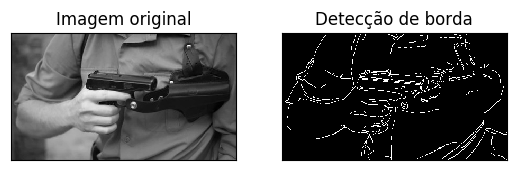
\includegraphics[scale=0.8]{img/canny.png}
  \caption{Comparação entre imagem de homem segurando uma pistola antes e depois do detector de bordas de Canny}
  \label{fig:canny}
\end{figure}

Uma outra possível solução se encontra nas redes neurais convolucionais, que representaram uma evolução na tecnologia de visão computacional. Essa topologia assemelha-se à de redes neurais profundas, porém conta, entre outros tipos de camada de suporte, com camadas convolucionais, em que cada neurônio representam um tipo de filtro aplicado à entrada da camada por meio da operação de convolução, demonstrada na figura \ref{fig:convolucao}.

\begin{figure}[ht]
  \centering
  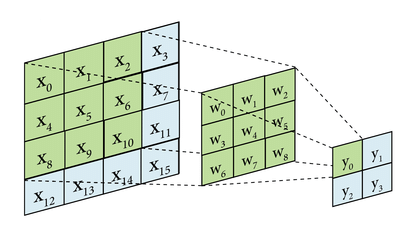
\includegraphics[scale=0.7]{img/convolucao.png}
  \caption{Diagrama mostrando a operação convolucional matricial, retirada de \citeyear{convolucao} \citeauthor{convolucao}}
  \label{fig:convolucao}
\end{figure}

Conforme o processo de aprendizagem supervisionada ocorre, a tendência é que os neurônios das camadas convolucionais passem a atuar como filtros que reagem especificamente a aspectos dos objetos presentes nas imagens que compõem o dataset de treinamento dessa rede. Na prática, isso significa que a matriz $\mathit{w_{i}}$ que na figura \ref{fig:convolucao} representa um neurônio de uma camada convolucional, terá valores mais altos em posições que correspondam a características desses objetos, como bordas, cantos e formas, e valores menores ou negativos em posições que não se encaixem nesse critério.

\begin{figure}[ht]
  \centering
  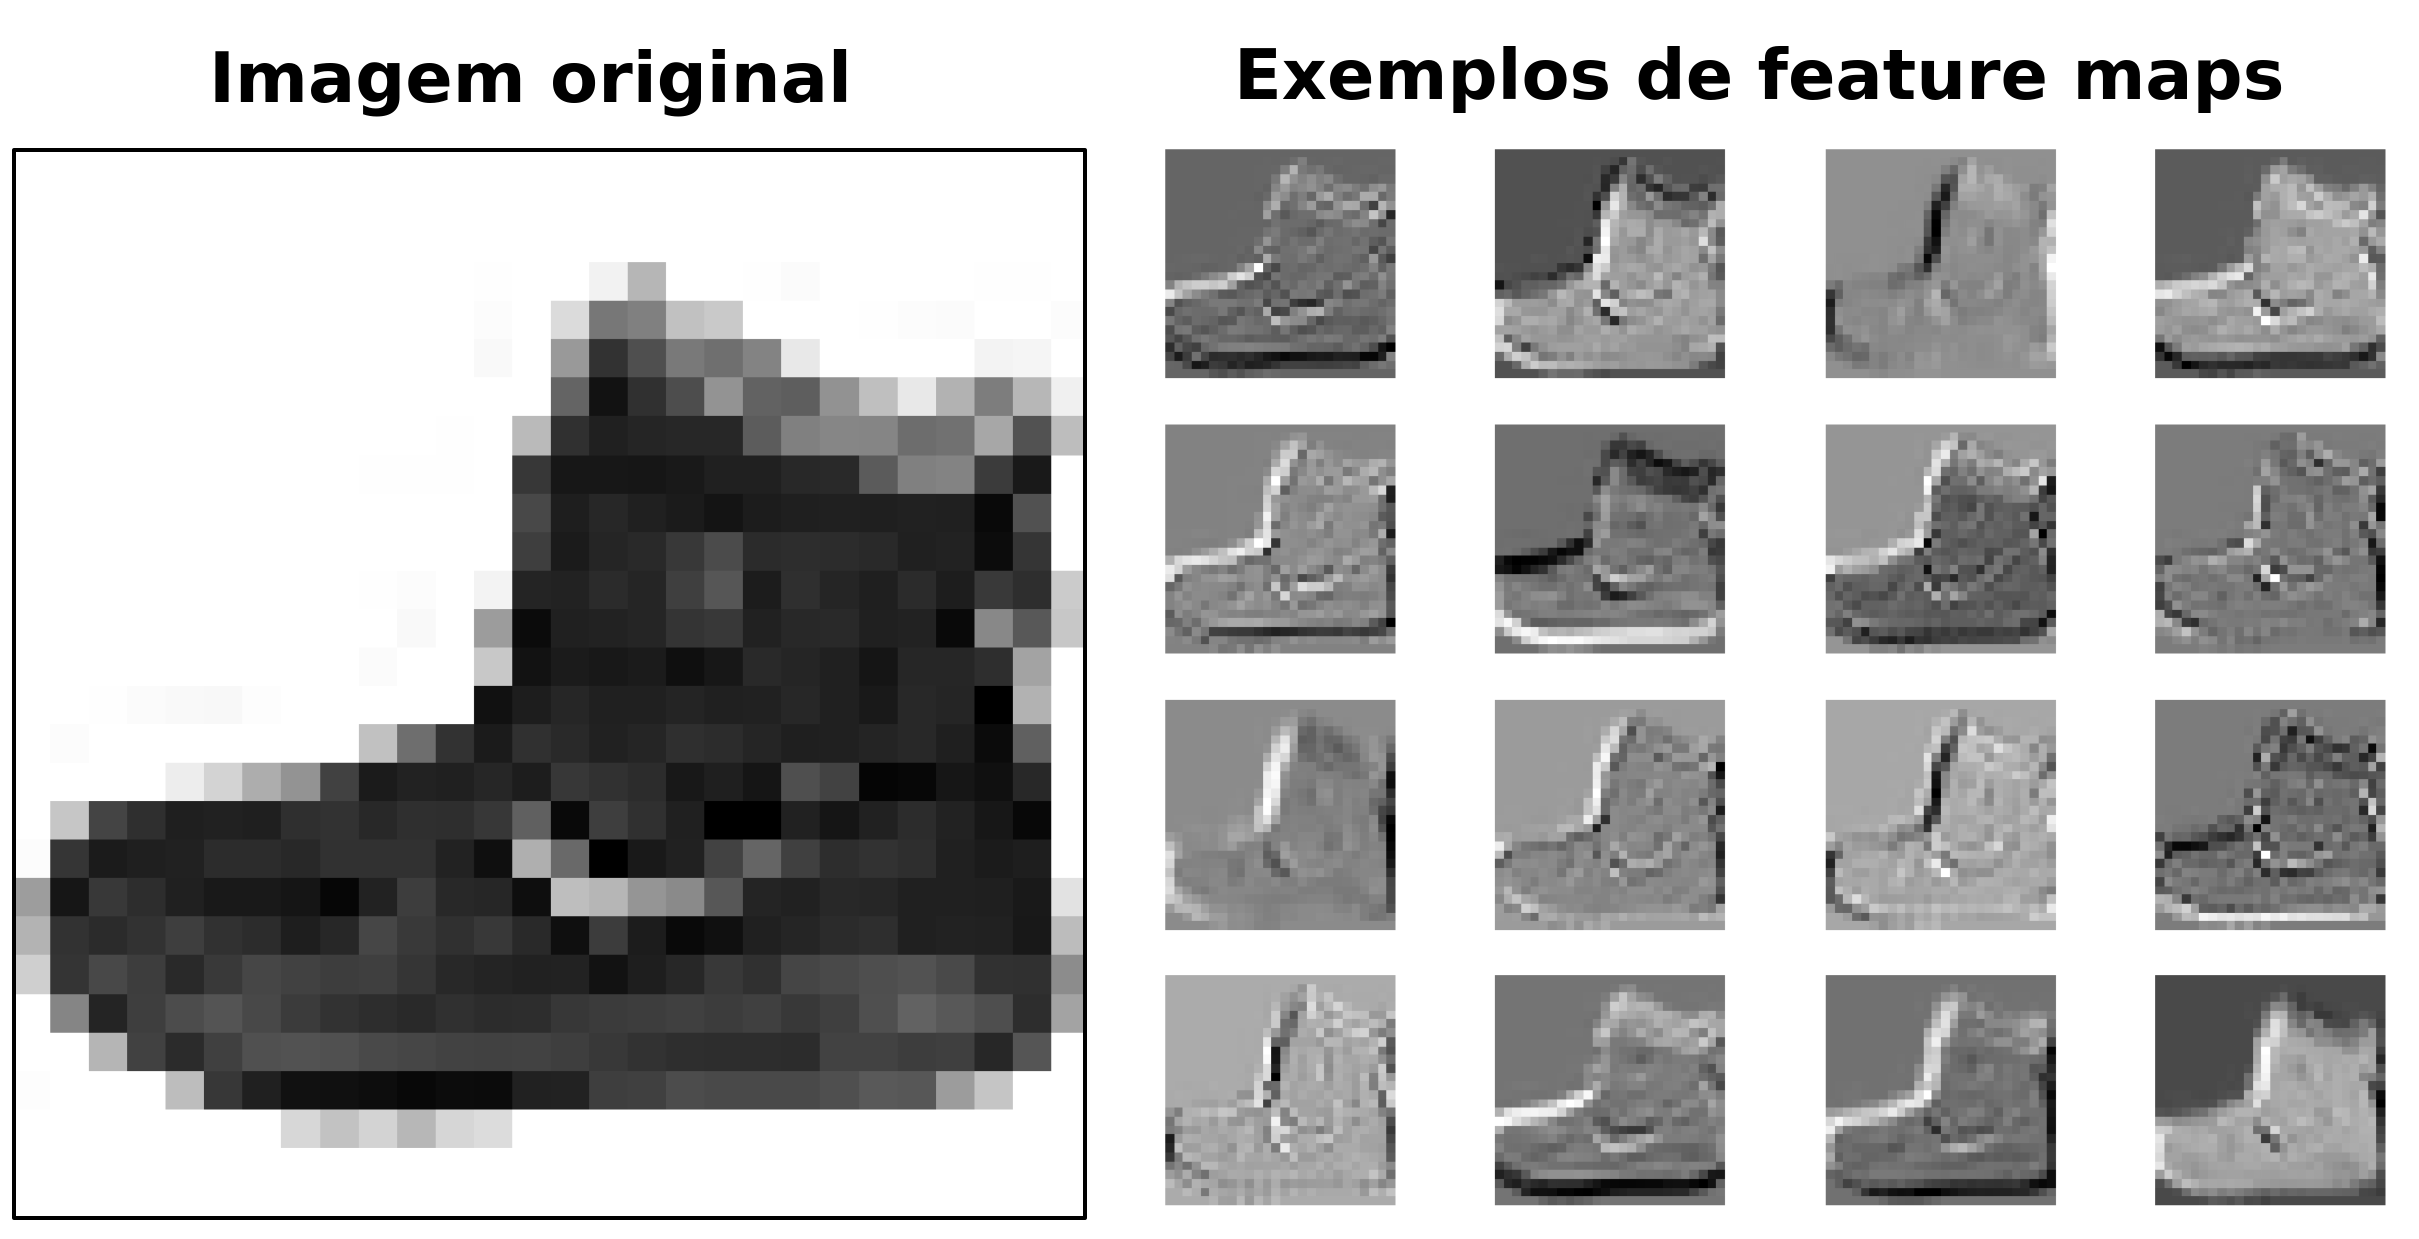
\includegraphics[scale=0.15]{img/featuremaps.png}
  \caption{Diagrama exemplificando \textit{feature maps} gerados a partir da convolução dos neurônios com a imagem da direita, retirado de \citeyear{featuremaps} \citeauthor{featuremaps} e traduzido para o português}
  \label{fig:featuremaps}
\end{figure}

Um exemplo do funcionamento dessas operações é mostrado na figura \ref{fig:featuremaps}. Do lado esquerdo observamos uma imagem de um sapato, que é alimentada em uma rede neural convolucional treinada para reconhecer esse tipo de objeto. Do lado direito observamos exemplos de chamados \textit{feature maps}, resultantes da convolução dos filtros (ou matrizes $\mathit{w_{i}}$) com a imagem de entrada. Ao analisar esses mapas, podemos observar que a convolução pareceu destacar certos aspectos do sapato, como suas bordas e seu formato geral. Notamos então que a reação positiva dos neurônios convolucionais quando alimentados com imagens de objetos que se assemelham a sapatos, evidencia o treinamento da rede como um todo para o reconhecimento desse tipo de objeto. As camadas convolucionais são posteriormente conectadas a um classificador, que dará uma resposta final sobre a classe à qual a imagem pertence.

Observamos, portanto, o avanço desse tipo de tecnologia em relação aos algoritmos descrios no início do capítulo. Enquanto ambos trabalham com extração de características das imagens, os algoritmos básicos de visão computacional se limitam a formas fixas e simples, enquanto o aprendizado profundo das redes neurais convolucionais é mais eficiente e mais flexível.

No entanto, mesmo a flexibilidade proporcionada pelas redes neurais convolucionais não é suficiente para o solucionamento do problema em questão. Ainda que tenhamos uma solução para a classificação de objetos, as redes neurais convolucionais não são o suficiente para cumprir o desafio da detecção de imagens, que supõe a classificação de objetos em posições quaisquer de um cenário sobre o qual não se tem controle, podendo o objeto estar presente ou não.

Trabalhos acadêmicos se propuseram a resolver esse problema. Inicialmente, foram adotadas abordagens de janela deslizante, onde, de maneira geral, classificadores (que podem se assemelhar ao descrito anteriormente ou não) eram aplicados em janelas de escalas variadas, que percorriam diferentes regiões da imagem por vez. Essa abordagem já é considerada ultrapassada, apresentando altos tempos de execução decorrentes da necessidade de se percorrer toda a área da imagem.

Uma abordagem mais avançada é a chamada de \textit{region proposals}, ou de proposição de regiões, onde certas porções da imagem que possuem uma maior probabilidade de conter um objeto são selecionadas a partir de um algoritmo auxiliar. Os algoritmos mais avançados que aplicam essa abordagem incoporam redes neurais convolucionais para a proposição de regiões, bem como uma cadeia de algoritmos auxiliares que permitem uma detecção rápida e com precisão satisfatória.

Atualmente, o trabalho de referência que aplica essa abordagem é \citeyear{fasterrcnn} \citeauthor{fasterrcnn}, que apresenta o algoritmo Faster R-CNN, aprimoramento da sequência que se iniciou com o algoritmo R-CNN apesentado em \citeyear{rcnn} \citeauthor{rcnn} e apresentou o subsequente Fast R-CNN em \citeyear{fastrcnn} \citeauthor{fastrcnn}. Em resumo, o trunfo do algoritmo Faster R-CNN é aplicar uma rede neural convolucional antes da rede de proposição de regiões, fazendo com que o classifcador atue sobre regiões selecionadas a partir de mapas de características extraídos da imagem original, e não da imagem em si. Essa redução de dimensionalidade resulta em tempos de detecção extremamente rápidos e suficientemente precisos, sendo a detecção rodada a 5 frames por segundo quando executada em uma GPU K40, apresentando uma média de precisões médias (\textit{mAP}) máxima de 42,7\%.

\begin{figure}[ht]
  \centering
  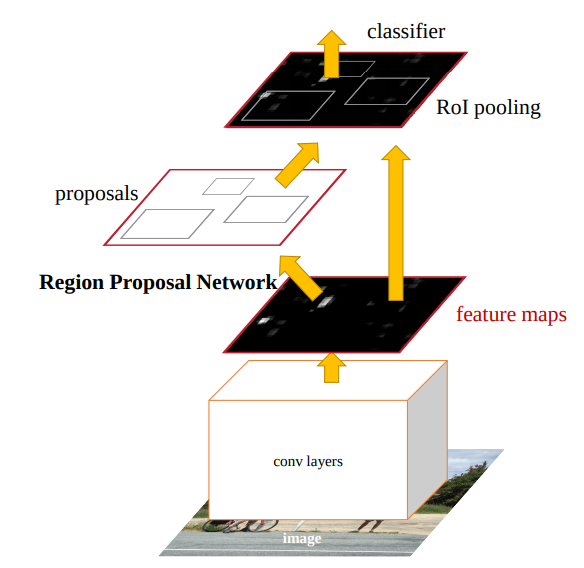
\includegraphics[scale=0.4]{img/fasterrcnn.png}
  \caption{Diagrama que demonstra a topologia do algoritmo Faster R-CNN, retirado de \citeyear{fasterrcnn} \citeauthor{fasterrcnn}}
  \label{fig:fasterrcnn}
\end{figure}

Por fim, abordagens mais recentes (e mais rápidas) procuram acelerar o processo ao tentar realizar todo o processo de detecção utilizando uma única rede neural. Os exemplos mais conhecidos são YOLOv3\cite{yolov3}, terceira iteração do algoritmo que é capaz de realizar uma taxa de frames por segundo máxima de 78 com média de precisões médias (\textit{mAP}) de 57,9\%; e SSD (Single Shot MultiBox Detector), apresentado em \citeyear{ssd} \citeauthor{ssd}, que apresentou taxa de frames por segundo máxima de 59, com média de precisões médias (\textit{mAP}) 74.3\%. Ambos os métodos possuem suas vantagem e desvantagens, com YOLOv3 fazendo propositalmente uma concessão de precisão em nome de uma maior velocidade.

O estudo e conhecimento desses métodos será essencial no momento de definir que algoritmos serão utilizados no sistema das câmeras de segurança, bem como os aspectos internos (como velocidade e precisão) e externos (como hardware) envolvidos em cada aplicação, fatores determinantes tanto na literatura existente como no projeto presente.

\section{Olmos: a referência em aplicação específica}

Sabemos quais as principais técnicas para detecção de imagens. No entanto, ainda não analisamos a literatura existente referente à aplicação específica com a qual estamos trabalhando: detecção de armas de fogo. São poucos os trabalhos que lidam com esse domínio e utilizam os algoritmos de estado da arte citados na seção anterior. Tomaremos como referência, portanto, \citeyear{olmos1} \citeauthor{olmos1}, desenvolvido por pesquisadores da Universidade de Granada.

O artigo também se inicia com uma breve recapitulação dos algoritmos de detecção de objetos mais recentes e com melhor performance. Em seguida, os pesquisadores procedem a comparar a performance de detecção de armas utilizando as abordagens de janela deslizante e de proposição de regiões. São apresentandos ao longo do processo os algoritmos utilizados, já bem estabelecidos, e, seguindo suas particularidades, os datasets de treinamento correspondentes utilizados que atuaram como os grandes responsáveis pela performance dos detectores.

Um conceito importante aplicado na execução da solução é o de \textit{transfer learning}. No treinamento de redes neurais desenvolvidas do zero, os pesos dos neurônios são inicializados de maneira aleatória, para que então o algoritmo de \textit{backpropagation} trabalhe para reduzir o gradiente da função de perda. No entanto, é possível inicializar a rede a ser treinada com um conjunto de pesos que seja relativo a alguma rede já treinada para algum outro fim de propósito semelhante. Ao fazer isso, apesar do risco de herdarmos viéses da rede já treinada, começamos o processo de treinamento com um gradiente da função de perda menor, e, portanto, esse terá seu tempo de execução reduzido. Na prática para o trabalho em questão, isso significa que aplicamos esse conceito a algoritmos originais, como Faster R-CNN, que são disponibilizados com pesos que permitem a detecção de múltiplas classes de objetos (baseados em datasets conhecidos como VGG-16) para adaptar o processo de detecção para focar apenas em armas. Como os domínios da rede já treinada e da rede pretendida são semelhantes (ambos tratam da detecção de objetos, sendo que um deles é apenas um caso mais específico), podemos inicializar o treinamento do detector de armas com os pesos para detecção do dataset VGG-16\cite{vgg16}, reduzindo o gradiente da função de perda e acelerando o processo de treinamento.

Um dos focos do trabalho, considerando que a solução desenvolvida também atuaria como um tipo de alarme para o uso de armas de fogo, é a redução de falsos positivos. Para a abordagem de janela deslizante, aumentar o número de classes do classificador pareceu ser a metodologia mais efetiva. Como esse percorre toda a imagem, e não só atua sobre as regiões mais relevantes, ao fazermos com que aprenda características de outros objetos além de armas de modo a também ser capaz de classificá-los, reduzimos as chances de uma janela da imagem ser classificada como uma arma, quando na verdade suas características se adequam mais a outra classe de objetos. Como resultado, o dataset de treinamento que melhor performou para a abordagem de janela deslizante continha 9261 imagens representando 102 classes, das quais apenas 200 eram relativas a armas.

A abordagem de proposição de regiões requer uma estruturação de dados diferente. Como uma única rede neural convolucional é responsável por determinar as regiões de interesse, é mais interessante que o treinamento se baseie em uma classificação binomial, ou seja, trabalhe em termos apenas da classificação ou não de um objeto como arma. Além disso, justamente pela proposição de regiões, o dataset para essa abordagem também precisa indicar \textit{bounding boxes}, que especificam o posicionamento do objeto na imagem. O dataset resultante contém 3000 imagens apenas de armas, bem como as \textit{bounding boxes} correspondentes.

\begin{figure}[ht]
  \centering
  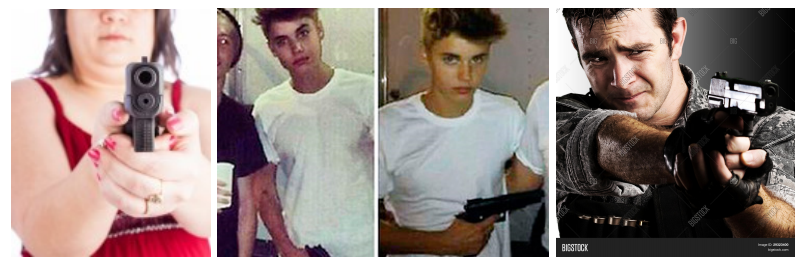
\includegraphics[scale=0.5]{img/dataset.png}
  \caption{Alguns exemplos do dataset para a abordagem de proposição de regiões, retirado de \citeyear{olmos1} \citeauthor{olmos1}}
  \label{fig:dataset}
\end{figure}

Como esperado, dado a evolução da pesquisa em algoritmos de detecção de imagem, a abordagem que apresentou melhor desempenho foi a de proposição de regiões. O modelo atingiu uma precisão de 84,21\%, com uma taxa de frames por segundo de 5,3, sendo capaz de realizar a detecção em, no mínimo, 200 milissegundos. Por fim, como o sistema ainda produzia um número pequeno de falsos positivos, e dado a natureza crítica de um sistema de alarme, os pesquisadores procuraram mitigar esse risco ao apenas acionar o alarme após a detecção em 5 frames consecutivos.

O trabalho de Olmos demonstra a efetividade de algoritmos de detecção, em especial os mais avançados, para o reconhecimento de armas de fogo. Além disso, os pesquisadores disponibilizaram publicamente os datasets utilizados, facilitando o trabalho de pesquisadores subsequentes. No entanto, dois fatores devem ser evidenciados: primeiramente, o fato de que todo o trabalho de treinamento e execução foi realizado utilizando aceleração por GPU, utilizando uma placa gráfica NVIDIA GTX 980, que conta com 4GB de memória. Em segundo lugar, o fato de que mesmo com a utilização desse recurso, a taxa máxima de frames por segundo foi de 5, que é suficiente para que a solução funcione em tempo real, mas ainda muito baixa se comparada com a taxa de frames padrão para captação de vídeo (entre 24 e 30).

De maneira geral, o resultado trazido pelo trabalho é promissor e apresenta um caminho a se seguir para a construção de nossa solução. No entanto, é importante notar as distinções entre o objeto deste trabalho e da pesquisa de Olmos. A mudança do paradigma de arquitetura para \textit{edge computing} terá consequências e acarretará em modificações, que serão descritas no próximo capítulo.

\chapter{Especificações de projeto}

Tendo passado por todo o conhecimento que constitui as bases necessárias para o desenvolvimento do projeto, precisamos estabelecer as especificações do mesmo, adaptando o estado atual da tecnologia ao contexto no qual nos propusemos a trabalhar e às novas arquiteturas propostas.

Dada a trajetória do avanço dos algoritmos de detecção de imagem, é óbvia a necessidade de utilização dos mais recentes e poderosos algoritmos, que apresentam uma performance mais próxima o possível do que seria uma situação ideal. No entanto, a escolha de algoritmo base apresenta \textit{trade-offs} específicos que precisam ser cuidadosamente considerados. Um fator essencial em todos os trabalhos revisados, e que é geralmente negligenciado, não só em trabalhos de detecção de imagem, mas de inteligência artifical como um todo, é a questão do hardware subjacente nos quais esses algoritmos são executados.

É de conhecimento geral que, atualmente, a computação para inteligência artificial se baseia fortemente em GPUs, devido às complexas operações matriciais envolvidas nos cálculos que compõem os algoritmos. Essa questão relacionada ao hardware não é, no entanto, abordada de maneira central nos trabalhos: a capacidade computacional para execução é, na maioria das vezes, um fator em segundo plano, que acompanha a complexidade do software na medida necessária. Em trabalhos como \citeyear{fasterrcnn} \citeauthor{fasterrcnn}, \citeyear{yolov3} \citeauthor{yolov3} e \citeyear{olmos1} \citeauthor{olmos1}, o tipo de GPU utilizado é mencionado apenas em passagem, e sua influência na performance do algoritmo é ignorada, apesar de ser um fator determinante nessa métrica.

Fato é, no projeto aqui proposto, estaremos trabalhando com um hardware projetado para sistemas embarcados, a placa Caninos Loucos, que comparativamente é muito menos potente do que o hardware em que as métricas publicadas para algoritmos de detecção de imagem se baseiam. Além disso, no estado atual de desenvolvimento do projeto Caninos Loucos, a placa utilizada não consegue executar aceleração por GPU, o que, se fosse possível, requeriria um esforço extra pois praticamente todas as bibliotecas e algoritmos de inteligência artificial que contam com esse recurso o baseiam na tecnologia proprietária CUDA, da NVIDIA.

Levando isso em consideração, é natural que procuremos, para esse hardware menos potente, o algoritmo com a melhor performance possível, visto que essa performance sofrerá perdas devido à execução em hardware mais simples. Parece, portanto, adequada a escolha de YOLOv3 como o algoritmo base para nosso trabalho, não só por ter apresentado as melhores métricas, mas também por apresentar uma arquitetura de funcionamento simplificada (avaliação por uma única rede) que se adequa melhor à execução em hardware simples.

Além disso, contamos com a conveniência da existência de um dataset de reconhecimento de armas publicado e disponível para uso, o mesmo utilizado \citeyear{olmos1} \citeauthor{olmos1}, o que poupa uma das etapas mais custosas e complicadas para treinamento de algoritmos de inteligência artificial: a coleta e tratamento de dados adequados para o problema. Tomaremos a escolha desse algoritmo e a disponibilidade do dataset como ponto de partida para a definição das especificações de projeto, descrevendo melhor funcionamentos específicos e resultados preliminares ao longo desse capítulo, bem como as escolhas decorrentes, que culminarão na estrutura final do projeto.

\section{YOLO}

O algoritmo YOLO (You Only Look Once) foi inicialmente apresentado em \citeyear{yolov1} \citeauthor{yolov1}, tendo sido aprimorado em \citeyear{yolo9000} \citeauthor{yolo9000}, numa versão chamada YOLO9000. No já mencionado \citeyear{yolov3} \citeauthor{yolov3}, ainda mais correções e melhorias são feitas a YOLO9000, resultando na versão atual do algoritmo, chamada YOLOv3.

Além da arquitetura simplificada de avaliação de rede única, o algoritmo possui a vantagem de trabalhar com dados no formato de \textit{bounding boxes}, que, apesar de requerer um maior trabalho para construção de um conjunto de treino, possuem a vantagem de prever não só a probabilidade de um objeto estar presente em uma imagem, mas também o seu posicionamento na mesma.

\subsection{Topologia e funcionamento}

Na versão mais recente, a detecção se baseia em uma única extrator de características, cuja topologia se encaixa nas chamadas \textit{Fully Convolutional Networks}, ou FCNs, redes neurais constituídas apenas de camadas convolucionais totalmente conectadas entre si. A rede que constitui esse extrator foi batizada de Darknet-53, denotando as 53 camadas convolucionais que a constituem, detalhadas na tabela \ref{tbl:darknet53}.

\begin{table}[ht]
  \centering
  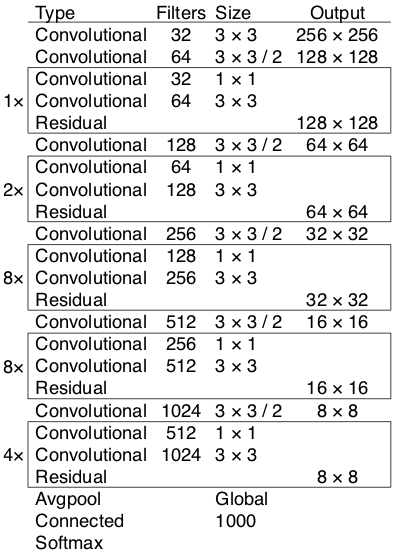
\includegraphics[scale=0.5]{img/darknet53.png}
  \caption{Tabela extraída de \citeyear{yolov3} \citeauthor{yolov3} descrevendo a topologia da rede Darknet-53, com colunas denotando, em ordem: tipo da camada, filtros, tamanho e \textit{output}.}
  \label{tbl:darknet53}
\end{table}

A camada convolucional é aplicada a cada camada a técnica de \textit{batch normalization}, onde são adicionados à normalização comum parâmetros multiplicativos e aditivos que também são treináveis, de forma a conter desequilíbrios nos pesos dos neurônios devido à diferença de escala dos dados. Além disso, os neurônios possuem função de ativação \textit{Leaky ReLU}, escolhida por apresentar ganhos de precisão e velocidade de treinamento.

O funcionamento do treinamento do algoritmo, de forma simplificada, pode ter seu funcionamento interpretado da seguinte forma: a imagem é dividida em células de mesma área, tomando as mesmas dimensões do mapa de características final extraído pela última camada convolucional da rede. Em seguida, como o conjunto de treino conta com a localização das \textit{bounding boxes}, encontramos a célula que contém o centro da \textit{bounding box} do objeto detectado.

\begin{figure}[ht]
  \centering
  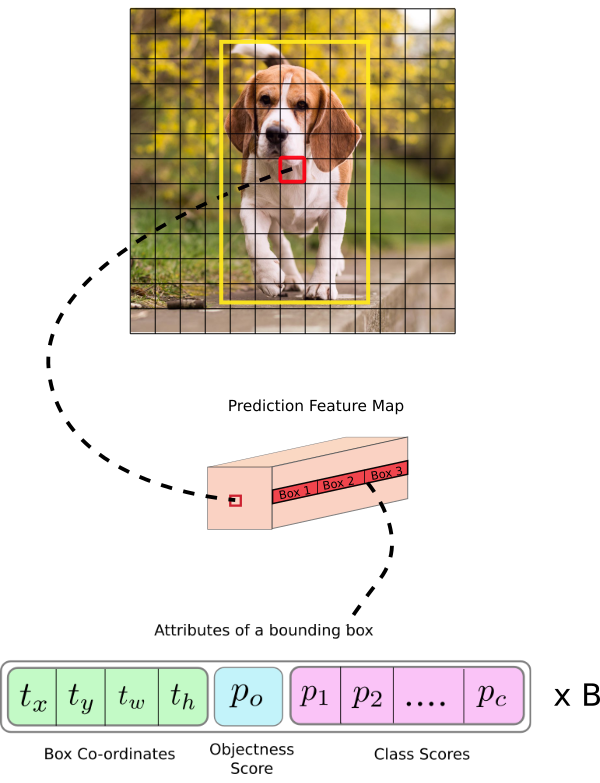
\includegraphics[scale=0.5]{img/yoloexplained.png}
  \caption{Diagrama representando a dinâmica simplificada de YOLO, retirado de \citeyear{yoloexplained} \citeauthor{yoloexplained}}
  \label{fig:yoloexplained}
\end{figure}

Essa célula do mapa de características será, portanto, responsável pela detecção daquele objeto e também pela predição da \textit{bounding box} correspondente, tendo seus parâmetros ajustados para tal. Esse processo é repetido para três escalas de imagem, garantindo uma margem para viabilidade do tamanho de objetos na cena.

Além do modelo completo, que leva o nome de YOLOv3, também é disponibilizado um modelo simplificado, chamado de YOLOv3-tiny, projetado com hardware menos poderoso em mente. Esse segundo modelo consiste em uma simplificação do modelo original por meio da remoção de algumas camadas, visando a diminuição do número de parâmetros, e, portanto, aumentando a velocidade de treinamento e de execução. A arquitetura modificada desse algoritmo é apresentada na tabela \ref{tbl:yolov3tiny}.

\begin{table}[ht]
  \centering
  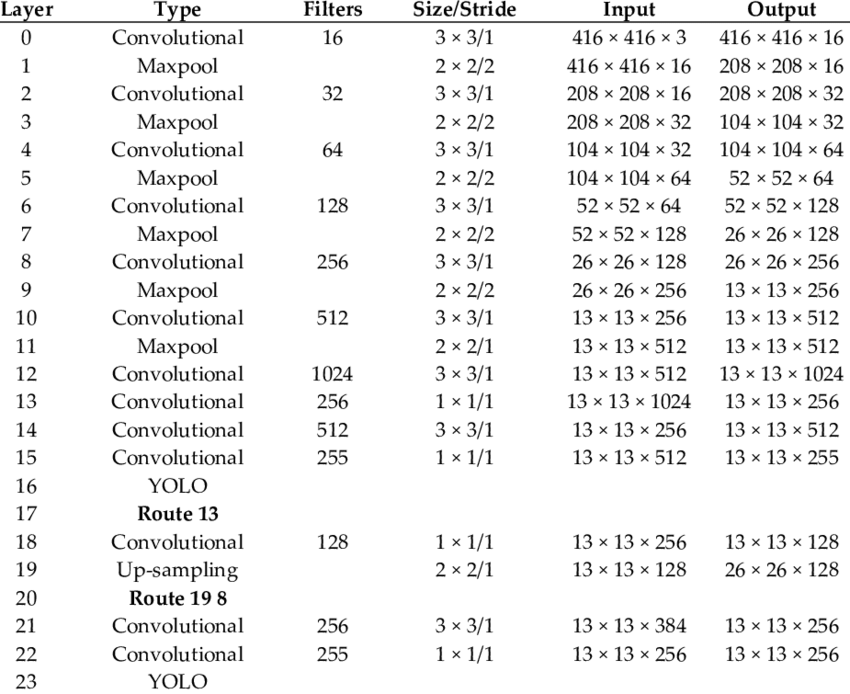
\includegraphics[scale=0.38]{img/yolov3-tiny.png}
  \caption{Tabela extraída de \citeyear{tfyolo} \citeauthor{tfyolo} descrevendo a topologia da rede modificada para o algoritmo YOLOv3-tiny}
  \label{tbl:yolov3tiny}
\end{table}

Como esse algoritmo parece se adequar a nosso uso de caso, realizaremos testes da versão mais recente, para garantir sua performance e adequação ao problema proposto. De antemão, podemos prever que arquiteturas semelhantes a de YOLOv3-tiny serão mais adequadas, devido à questão levantada no início do capítulo de que o \textit{baseline} de hardware para esse tipo de algoritmo na literatura é muito alto.

\subsection{Testes iniciais e resultados}

Buscando iniciar o desenvolvimento do projeto e também confirmar a viabilidade da escolha do ponto de partida, foram realizados testes iniciais, de maneira simplificada. Como o foco dessa subseção do trabalho é a análise dos resultados e suas implicações para as especificações do projeto, focaremos aqui nos mesmos, com as metodologias e processos sendo descritos no capítulo 4.

A versão do algoritmo publicada e disponibilizada pelos pesquisadores online conta com pesos pré-treinados para o dataset COCO\cite{coco}, sendo a versão padrão da rede capaz de detectar múltiplas classes de objetos. Inicialmente, tentou-se analisar de forma preliminar o tempo de detecção nessa configuração, para obter-se uma métrica de base. Buscando se aproximar das condições de execução da Caninos Loucos, ou seja, rodando apenas em CPU, testes de detecção iniciais foram realiados em um processador Intel Core i5 de 64 bits. Nesse caso, os tempos de detecção para imagens únicas girou em torno de 28 segundos, um tempo muito aquém do esperado, principalmente ao considerar que \citeyear{yolov3} \citeauthor{yolov3} apresenta performance de 78 frames por segundo para a rede Darknet-53, correspondendo a um tempo de detecção de aproximadamente 13 milissegundos.

É evidente que essa diferença pode ser atribuída à falta de aceleração por GPU nas condições de teste, demonstrando mais uma vez o fato de que condições de hardware não são consideradas no estabelecimento de métricas de performance. O tempo de detecção obtido, que corresponde a uma taxa de 0,035 frames por segundo, inviabiliza a aplicação do algoritmo para detecção em tempo real executada em CPU. Sendo assim, foi necessário a busca por alternativas.

Utilizando-se a versão simplificada da rede disponibilizada pelos pesquisadores, chamada de YOLOv3-tiny, a performance obtida apresentou grande melhora. Tempos de detecção individuais giraram em torno de 1,1 segundos, o que aproxima a performance do algoritmo para um caso de uso de tempo real, no entanto ainda sem apresentar viabilidade para tal. Vale notar que, ao utilizarmos o modelo simplificado do algoritmo, optamos por priorizar a velocidade de processamento em detrimento da precisão de detecção. Apesar do resultado obtido não ser ideal, uma taxa de aproximadamente 1 frame por segundo ainda permite que algumas modificações de arquitetura sejam feitas para que essa taxa seja compensada, como por exemplo a utilização de múltiplas câmeras em uma mesma área, com suas detecções combinadas. 

No entanto, ao efetivamente colocar a teste a performance do algoritmo na placa Caninos Loucos, o resultado foi ainda pior: uma única detecção demorou, em média, 45 segundos, o que pode ser explicado pelo poder computacional da CPU embarcada da placa ser, na prática, muito menor do que o processador utilizado nos primeiros testes.. Essa taxa de frames por segundo completamente inviabiliza a execução de YOLOv3 na borda computacional.

O único caminho possível é, portanto, caminhar em direção a uma simplificação ainda maior do modelo, estando atento à concessão de precisão que acompanha esse processo. Podemos, porém, de forma complementar, compensar a queda na precisão por meio de alterações na arquitetura, utilizando técnicas já conhecidas de combinação de algoritmos para melhorar a precisão do sistema como um todo. Precisaremos, portanto, encontrar uma maneira de simplificar o algoritmo para além da redução feita em YOLOv3-tiny, para em seguida desenhar uma nova arquitetura que acomode as novas características do sistema.

\subsection{YOLO-LITE e modelo simplificado}

Esgotados os recursos presentes nos artigos publicados pelos idelizadores do framework YOLO, recorremos à outros estudos realizados na academia em relação ao algoritmo. Em \citeyear{yololite} \citeauthor{yololite}, pesquisadores estadunidenses deram um passo atrás e, baseando-se na versão simplificada da segunda iteração do algoritmo, YOLOv2-tiny, testaram diferentes alterações e simplificações adicionais à topologia, de modo a otimizar o funcionamento do algoritmo para execução em CPU.

A métrica estabelecida como objetivo foi de obter uma taxa de frames por segundo próxima de 10 sem aceleração por GPU, bem como um \textit{mAP} de 30\%. Em seguida, foram projetadas e treinadas diferentes configurações de redes simplificadas, que foram testadas de acordo com essa métrica no dataset Pascal VOC 2007\cite{pascalvoc}. O modelo com melhor performance foi então retreinado, utilizando a técnica de \textit{transfer learning}, para o dataset COCO\cite{coco}, apresentando uma performance ainda melhor.

\begin{table}[ht]
  \centering
  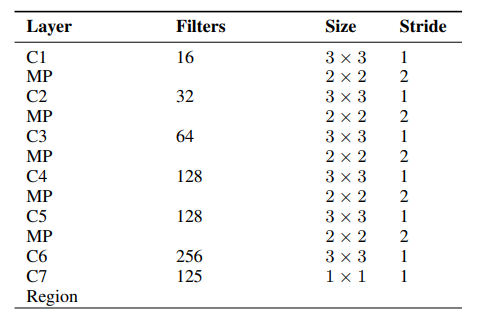
\includegraphics[scale=0.55]{img/yololite.png}
  \caption{Tabela extraída de \citeyear{yololite} \citeauthor{yololite} descrevendo a topologia da rede que melhor performou para as métricas estabelecidas.}
  \label{tbl:yololitearchitecture}
\end{table}

A arquitetura de melhor performance, e que foi selecionada para levar o nome, por fim, de YOLO-LITE está apresentada na tabela \ref{tbl:yololitearchitecture}. Notamos, em relação à topologia original apresentada na tabela \ref{tbl:yolov2tiny}, a eliminação de camadas convolucionais bem como a redução do número de filtros das restantes, além da remoção de uma camada de \textit{Max Pooling} na entrada da rede, reduzindo o número total de parâmetros da rede. Além disso, deixou-se de aplicar a técnica de \textit{batch normalization}, que apesar de ser considerada um ponto positivo em YOLOv3, não apresentou ganhos de performance significativos para essa versão da rede simplificada.

\begin{table}[ht]
  \centering
  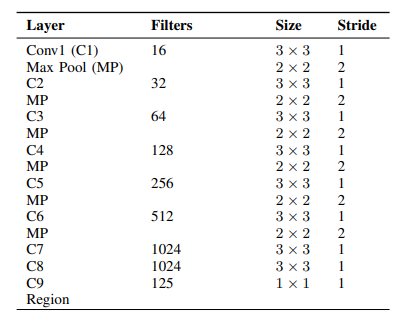
\includegraphics[scale=0.66]{img/yolov2tiny.png}
  \caption{Tabela extraída de \citeyear{yololite} \citeauthor{yololite} descrevendo a arquitetura original da rede YOLOv2-tiny}
  \label{tbl:yolov2tiny}
\end{table}

O modelo final acabou performando ainda melhor, atingindo a marca de 10 frames por segundo sendo executado em um \textit{browser} web, e chegando a 21 quando executado em uma CPU tradicional. Além disso, o modelo escolhido apresentou uma média de precisões médias (\textit{mAP}) de 33,77\%. Sendo assim, a utilização de YOLO-LITE parece, finalmente, se adequar a nosso caso de uso com uma performance significativa. Apesar da queda brusca de precisão no algoritmo, procuraremos compensá-la com mudanças na arquitetura.

\section{Nova arquitetura}

Estabelecidas as limitações encontradas devido à iniciativa de mudança de arquitetura para o paradigma de \textit{edge computing}, precisamos contorná-las de forma a não comprometer ainda mais a precisão do algoritmo. Temos como única certeza e ponto de partida, inicialmente, que a execução completa de YOLOv3 na borda computacional é inviável. Sendo assim, a ideia aqui é que a borda computacional execute algoritmos de menor precisão, fazendo uma espécie de pré-processamento das imagens, assim selecionando casos mais relevantes para uma análise mais profunda feita utilizando o já mencionado YOLOv3, em hardware que seja capaz de processá-lo de maneira suficientemente rápida.

Na área de aprendizado de máquina, são acomodadas embaixo do termo guarda-chuva \textit{ensemble learning} as técnicas que reúnem diversos algoritmos de classificação de modo a combinar seus resultados para obter uma precisão maior. Essa área se baseia no princípio popularmente conhecido como "sabedoria das multidões", que afirma que grandes grupos de indivíduos são, coletivamente, capazes de tomar decisões melhores se comparados aos indivíduos por si só. O princípio ganha força na ideia de que a heterogeneidade entre os indivíduos garante que ao mesmo tempo que ideias comuns sejam amplificadas, aspectos diversos também sejam considerados, podendo, em certos casos, inclusive contrabalancear excessos.

Em um escopo técnico, o princípio representa a capacidade de diferentes modelos de aprender características diferentes dos dados de treinamento em decorrência das suas particularidades matemáticas. Ao combiná-los, estaríamos ampliando então a quantidade de características aprendidas, resultando em um modelo que é, no mínimo tão preciso quanto o melhor modelo entre aqueles que foram combinados, e provavelmente podendo superá-lo. Essa combinação é especialmente útil quando tratamos de um conjunto grande de \textit{weak learners}, ou algoritmos de baixa precisão, o que é uma forma de se melhorar a performance de algoritmos de inteligência artificial quando se tem poucos dados para treinamento.

O problema representado pela velocidade de detecção de YOLOv3 na Caninos Loucos se encaixa, em partes, ao paradigma descrito aqui até então. Podemos considerar um detector único como um \textit{weak learner}, tanto pela queda de precisão representada pela utilização do modelo simplificado YOLOv3-tiny quanto pela baixa taxa de frames por segundo, que faz com que, considerando a detecção de forma agregada ao longo do tempo, essa precisão aparente ser menor ainda.

No entanto, em um problema mais simples, tradicionalmente para a criação de um \textit{ensemble}, seriam aplicados a um conjunto de dados, por exemplo, mais de um tipo de classificador, que seriam combinados utilizando técnicas de \textit{bagging} ou \textit{bootstrapping}. A modelagem matemática específica dessas técnicas não se aplica especificamente ao caso presente devido à presença do detector de imagens, nos fazendo recorrer a um modelo novo e alternativo, porém inspirado da arquitetura de \textit{ensemble learning}.

\begin{figure}[ht]
  \centering
  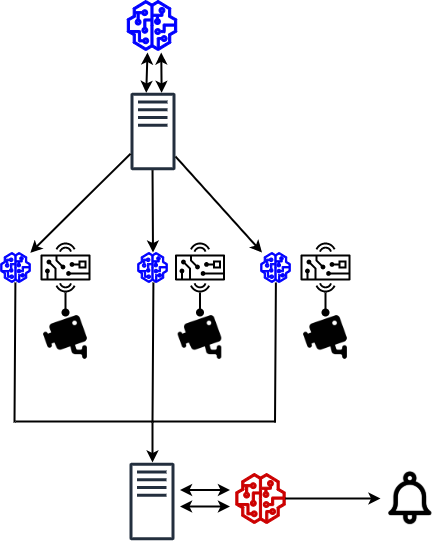
\includegraphics[scale=0.7]{img/novaarquitetura.png}
  \caption{Diagrama demonstrando, de maneira simplificada, a nova arquitetura proposta para solução do problema}
  \label{fig:novaarquitetura}
\end{figure}

Na figura \ref{fig:novaarquitetura}, é apresentada a proposta de arquitetura para a solução, desenhada a partir da já estabelecida arquitetura de edge computing. Todo o início do fluxo é igual ao proposto anteriormente, com um servidor central de grande capacidade dedicado ao treinamento do algoritmo de detecção de imagens distribuindo o modelo pronto para as localidades das câmeras, que são responsáveis pelo trabalho de detecção em cima das imagens. No entanto, a ideia central dessa nova proposta é a utilização de mais de um conjunto consistindo em uma câmera e uma placa Caninos Loucos por localidade no mundo físico, combinando as detecções, ainda que relativamente lentas e imprecisas de \textit{n} câmeras atuando conjuntamente para a obtenção de alertas mais precisos.

As câmeras estariam posicionadas a diferentes ângulos de uma mesma cena, de certa forma incorporando o aspecto heterogêneo que um \textit{ensemble} tradicional apresenta. Além disso, a presença de mais câmeras permite que a frequência de captura de probabilidades de detecção seja multiplicada por \textit{n} de forma global, mitigando o problema atualização de dados em uma câmera individual a uma frequência muito menor que a de captura de imagem. Seguindo a lógica de um \textit{ensemble}, devemos combinar as probabilidades obtidas pela câmera de alguma forma, o que nos leva a parte inferior do fluxo no diagrama da figura \ref{fig:novaarquitetura}. À medida em que as múltiplas câmeras presentes em uma mesma cena calculam probabilidades de detecção a partir de YOLOv3, essas probabilidades são enviadas a um algoritmo classificador que, baseado nas \textit{n} probabilidades recebidas, classifica de maneira definitiva a ocorrência em uso ou não de arma de fogo. Esse algoritmo, na arquitetura proposta, é representado por um segundo servidor externo contendo o modelo responsável pela classificação.

A opção pelo posicionamento desse modelo em uma estrutura externa e não na borda computacional em si decorre, principalmente do conjunto de dados que se torna necessário para que esse classificador funcione. Para que treinemos o classificador, precisamos de um conjunto de treino que relacione \textit{n} probabilidades detectadas por YOLOv3 em diferentes ângulos e uma confirmação de se aquele agrupamento de probabilidades representa uma ocorrência real ou não. Seja pelo número único de \textit{n} câmeras em cada área ou pelas probabilidades produzidas por essas câmeras variar em função de fatores como posicionamento, luminosidade, movimentação e pontos cegos, não existe um único conjunto de dados que sirva pra treinar um único modelo genérico de classificador que funcione em todas as localidades. É necessário então que sejam construídos conjuntos de dados e classificadores individuais para cada conjunto de \textit{n} câmeras que atuem sobre uma mesma área.

Esse segundo servidor central serviria, portanto, como ponto centralizador da coleta de dados para construção do conjunto de treino, da execução de rotinas de treinamento e atualização de modelos, e da classificação em si. Como os dados de treinamento constituem o que se chama de \textit{unlabeled data}, ou dados não identificados, a ideia é que este servidor esteja conectado às estações de trabalho de atendentes de serviços de emergência. Ao detectar uma probabilidade mínima da existência de armas na imagem, as câmeras, além de enviar ao servidor a probabilidade correspondente, enviariam também o conteúdo das imagens da câmera referente àquela probabilidade. Essas informações seriam exibidas em um \textit{dashboard} operado pelos atendentes, que seriam responsáveis por, em um momento inicial, classificar manualmente os dados até que se obtenha o suficiente para o treinamento de um modelo autônomo preciso o suficiente.

É importante notar que essa nova arquitetura acaba fazendo com que o projeto se distancie da arquitetura ideal de \textit{edge computing} discutida no capítulo inicial. De maneira semelhante, a necessidade da classificação manual de dados por operadores humanos para a criação dos modelos classificador se distancia da situação ideal de um algoritmo 100\% autossuficiente. Essas são concessões feitas de maneira a garantir a viabilidade do projeto dado o estado tecnológico atual. Defendemos, no entanto, que mesmo na nova forma apresentada, a arquitetura proposta ainda pode ser classificada como de \textit{edge computing}, visto que uma boa parte do trabalho computacional é executado na borda. Esse trabalho computacional distribuído acarreta em uma redução de dimensionalidade, fazendo com que se deixe de trafegar um volume massivo de dados relativos à vídeo, e passemos a trafegar dados que, no máximo, consistirão de um inteiro representando uma probabilidade e uma única imagem pontual, referente à um momento espaçado no tempo.

A nova arquitetura, portanto, é eficaz em mitigar os problemas causados pela distância entre o hardware disponível e aquele tido como base para a performance de algoritmos de detecção, enquanto também endereça questões que permeiam os problemas resolvidos pelo paradigma de \textit{edge computing}. Sendo assim, essa é a arquitetura a ser implementada, representando esse balanço entre os fatores envolvidos.

\section{Classificadores lineares e SVMs}

A única estrutura que resta a ser definida no projeto é a do classificador que, a medida em que dados suficientes forem coletados, passará a determinar de forma definitiva a ocorrência de uso de armas. O primeiro passo é, portanto, escolher um tipo de modelo que se adeque às características dos dados que se quer classificar. Como estamos trabalhando com probabilidades de detecção, temos um caso óbvio onde a classificação é negativa e que ocorrerá na maior parte do tempo: quando nenhuma das câmeras detecta a presença de uma arma. Sendo assim dependendo do tipo de modelo utilizado, o risco de sobreajuste é alto, pois ou estaremos aplicando um viés muito grande para casos em que todas as probabilidades são nulas; ou, excluindo os casos onde isso acontece, treinando o modelo apenas com exemplos positivos, o que também não gera um resultado satisfatório.

Como estamos falando de apenas quatro valores (referentes às quatro probabilidades) e duas classes possíveis (uso de arma ou não), um classificador linear parece adequado. Classificadores lineares, na prática, atuam como divisores do espaço geométrico dos dados, separando-no em regiões correspondentes à diferentes classes e que são delimitadas por fronteiras lineares (retas, hiperplanos tridimensionais, e assim por diante).

Um conjunto de clasificadores lineares que está entre os mais utilizados é o das \textit{Support Vector Machines}, ou SVMs na abreviação. Primeiramente, o algoritmo encontra uma provável fronteira que separe completamente os pontos de cada classe. Em seguida, essa fronteira é otimizada por um processo chamado otimização de margem, onde as distâncias entre os pontos e a fronteira (chamadas de vetores de suporte, dando origem ao nome do algoritmo) são maximizadas. Sendo assim, essa reta classifica da maneira mais eficiente possível novas observações com base nos pontos utilizados para o treinamento.

\begin{figure}[ht]
  \centering
  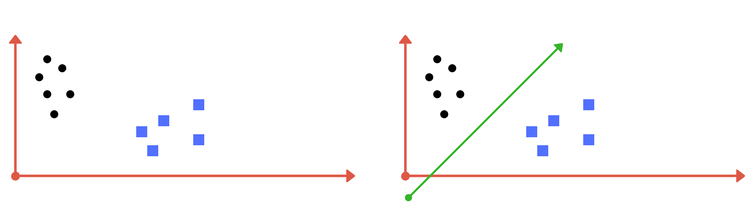
\includegraphics[scale=0.6]{img/svmlinear.jpg}
  \caption{Funcionamento simplificado de uma \textit{Support Vector Machine} onde os dados brutos são linearmente separáveis, retirado de \citeyear{svmimagens} \citeauthor{svmimagens}}
  \label{fig:svmlinear}
\end{figure}

No entanto, em processos onde os pontos de cada classe não são separáveis por uma reta, essa metodologia, por si só, passa a não funcionar. Para resolver esse problema, as SVMs se valem de transformações algébricas lineares denominadas \textit{kernels}, que transformam os dados para um espaço de dimensões onde os pontos se tornem linearmente separáveis.

\begin{figure}[ht]
  \centering
  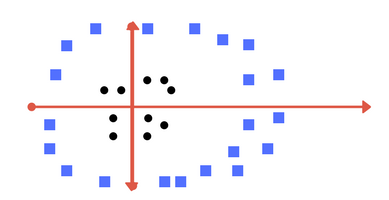
\includegraphics[scale=0.6]{img/svmnaolinear.png}
  \caption{Neste exemplo, os dados apresentados de diferentes classes não podem ser separados por uma reta. Retirado de \citeyear{svmimagens} \citeauthor{svmimagens}}
  \label{fig:svmnaolinear}
\end{figure}

Um exemplo pode ser observado na figura \ref{fig:svmnaolinear}, onde os dados, posicionados em um plano bidimensional, não podem ser separados utilizando uma reta. No entanto, se aplicarmos uma transformação como a demonstrada na figura \ref{fig:svmkernel}, observamos que em um espaço dimensional mais elevado, os dados transformados são linearmente separáveis. Observamos o funcionamento da técnica ao constatar que, transformando o hiperplano da fronteira de volta para o plano bidimensional original, o mesmo toma a forma de um círculo, atendendo às necessidades da disposição dos dados.

\begin{figure}[ht]
  \centering
  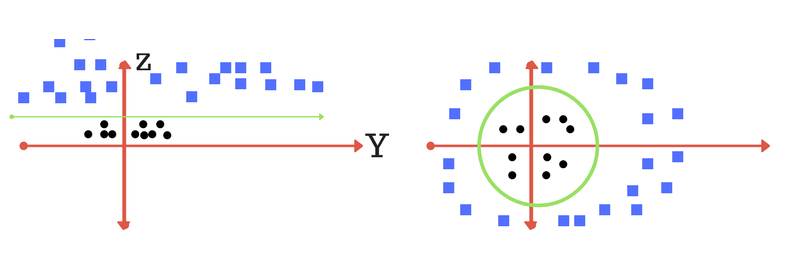
\includegraphics[scale=0.6]{img/svmkernel.jpg}
  \caption{Figura mostrando os dados de exemplo sendo linearmente separados após a aplicação de um \textit{kernel}, e o resultado convertido para o espaço dimensional original, retirada de \citeyear{svmimagens} \citeauthor{svmimagens}}
  \label{fig:svmkernel}
\end{figure}

O \textit{kernel} mais comumente utilizado em conjunto com esse tipo de algoritmo é chamado de \textit{Radial Basis Function}, ou RBF, em abreviação. A definição que calcula as relações de maior dimensionalidade entre duas observações é apresentada em \ref{rbfkernel}.

\begin{equation}
  K(a,b) = e^{-\gamma \times (a-b)^{2}}
  \label{rbfkernel}
\end{equation}

Apesar de sua dedução matemática ser complicada e longa, o funcionamento do \textit{kernel} se baseia, de maneira simplificada, na distância entre uma nova observação e as observações existentes. Sendo assim, dimensionada pelo parâmetro $\mathit{\gamma}$, as novas observações podem ser mais ou menos associadas à sua distância até as observações já existentes. Esse \textit{kernel} apresenta o melhor resultado, no geral, e portanto é o mais utilizado.

As SVMs também extrapolam essa lógica para espaços dimensionais maiores, o que significa, na prática, que podemos aplicar esse mesmo modelo para observações que contenha quantas características desejarmos, separando-as em duas classes. Dado o tipo de classificação que precisamos realizar, a aplicação de uma SVM às \textit{n} previsões enviadas pela câmera para classificarmos uma ocorrência em uso ou não de armas de fogo parece adequado.

\chapter{Solução final e resultados}

Com todos os parâmetros estabelecidos, prosseguimos para a prototipação de uma solução final. Este capítulo descreverá os passos executados para se chegar nessa solução final, bem como os resultados obtidos em cada etapa.

Primeiramente, adaptaremos a variação do algoritmo YOLO, YOLO-LITE, para o nosso caso de uso, aplicando a técnica de \textit{transfer learning} para treinar a rede utilizando o dataset de \citeyear{olmos1} \citeauthor{olmos1}. Em seguida, executaremos essa versão do algoritmo na placa Caninos Loucos, fazendo uma captura contínua que, ao detectar uma probabilidade suficientemente alta de uso de pistola, enviará esse dado e a imagem estática da cena correspondente. Esses dados serão alimentados para uma API, que será responsável por coletá-los e, com a ajuda de classificação manual, construir ao longo do tempo um classificador inteligente que se torne autossuficiente. O último passo a ser descrito é a caracterização desse classificador e seus usos futuros.

Para todos os passos aqui descritos, estaremos assumindo um valor fixo para \textit{n}, o número de câmeras por área, de 4. Também estaremos focando o desenvolvimento, de forma prototipada, para apenas uma área, tomando cuidado para facilitar a generalização e replicação do trabalho para um sistema integrado maior no futuro.

\section{Adaptação de YOLO para o caso de uso}

Como observamos ao longo dos capítulos mais teóricos desse trabalho, algoritmos de \textit{deep learning}, por lidar com operações matriciais com muitos parâmetros envolvidos, requerem uma capacidade computacional alta não só para serem executados, mas também, e especialmente, para serem treinados. Sendo assim, como observado desde a primeira arquitetura de \textit{edge computing} proposta, e reforçado pela nova arquitetura definitiva, o treinamento de um algoritmo de visão computacional da complexidade de YOLO precisa ser realizado em hardware potente independete de onde será executado para que consigamos atingir tempos de treinamento viáveis.

Sendo assim, optamos por utilizar o ambiente em nuvem Google Colab\cite{colabblog}, que disponibiliza hardware especializado em inteligência artifical para uso público e gratuito, por meio de sessões de máquinas virtuais. Como fica explícito na tabela \ref{tbl:googlecolab}, as especificações das máquinas disponibilizadas correspondem a um nível ótimo para treinamento de algoritmos, garantindo que consigamos trabalhar com tempos relativamente curtos para as tarefas.


\begin{table}[]
\centering
\begin{tabular}{|c|l|l|l|l}
\cline{1-4}
\multirow{2}{*}{CPU} & \multicolumn{3}{l|}{Processador Intel Xeon de 1 core \textit{hyperthreaded}} &  \\ \cline{2-4}
                     & \multicolumn{3}{l|}{2,3GHz, 45MB de cache}                          &  \\ \cline{1-4}
\multirow{3}{*}{GPU} & \multicolumn{3}{l|}{NVIDIA Tesla K80}                               &  \\ \cline{2-4}
                     & \multicolumn{3}{l|}{2496 cores CUDA}                                &  \\ \cline{2-4}
                     & \multicolumn{3}{l|}{12GB de memória VRAM GDDR5}                     &  \\ \cline{1-4}
Memória RAM          & \multicolumn{3}{l|}{12,6GB disponíveis}                             &  \\ \cline{1-4}
\end{tabular}
\caption{Especificações do hardware disponibilizado pela plataforma Google Colab}
  \label{tbl:googlecolab}
\end{table}

Para que apliquemos a técnica de \textit{transfer learning}, primeiro precisamos ajustar alguns parâmetros de treinamento da rede base de YOLO-LITE, a rede escolhida. Ajustamos o número de classes para 1, correspondente à unica classe que queremos identificar (armas), substituindo as 20 classes do modelo inicial. Como consequência, também ajustamos o número de filtros da última camada convolucional, de acordo com a equação \ref{filters}, onde \textit{f} é o número de filtros, \textit{n} é o número de clusters e \textit{c} é o número de classes, fazendo com que o novo número de filtros seja 30.

\begin{equation}
  f = n \times (c + 5)
  \label{filters}
\end{equation}

Em seguida, executamos um script para conversão dos dados de \textit{bounding boxes} do dataset de \citeyear{olmos1} \citeauthor{olmos1} do formato em extensão \textit{.xml} e com metadados extras para o formato \textit{.txt} simplificado utilizado pelo framework YOLO. Em seguida, separamos esse dataset em um conjunto de treino e de teste, seguindo a proporção de 80\% e 20\%, respectivamente. Considerou-se que a divisão de maneira aleatória é adequada nesse caso, considerando que o dataset possui imagens de aspecto diferenciado distribuídas por toda a sua extensão, e que as imagens, como dados, são variáveis independentes entre si.

Por fim, apenas executamos o treinamento do detector, apontando o dataset modificado como conjunto de treino e inicializando os pesos da rede com os pesos resultantes de \citeyear{yololite} \citeauthor{yololite}, treinado para detectar objetos do dataset COCO\cite{coco}. Dessa forma, o processo de treinamento parte de um ponto onde o gradiente de erro será muito menor do que um processo com os pesos incializados de maneira aleatória. Para tal, executamos o comando:

\begin{lstlisting}
./darknet detector train "obj.data" "cfg/yolo-lite.cfg" "yolo-lite.weights" -dont_show
\end{lstlisting}

Onde \textit{obj.data} é o arquivo que define o número de classes e o dataset de treino, \textit{cfg/yolo-lite.cfg} define a topologia da rede a ser treinada, seguindo o modelo demonstrado na seção 3.1.3, e \textit{yolo-lite.weights} corresponde aos pesos já treinados para o dataset Pascal VOC do projeto original.

O algoritmo foi treinado por aproximadamente 8 horas. Isso correspondeu a 257.200 iterações de treinamento, sendo que 247.401 delas são referentes aos pesos de treinamento para o dataset Pascal VOC 2007 pré-disponibilizados por \citeyear{yololite} \citeauthor{yololite}, e as 15.799 restante ao \textit{transfer learning} realizado utilizando o dataset presente em \citeyear{olmos1} \citeauthor{olmos2}.

\begin{table}[h]
\centering
\begin{tabular}{lllll}
\cline{1-2}
\multicolumn{1}{|l|}{\textbf{mAP}}       & \multicolumn{1}{l|}{45,84\%} &  &  &  \\ \cline{1-2}
\multicolumn{1}{|l|}{\textbf{Precisão}}  & \multicolumn{1}{l|}{30\%}    &  &  &  \\ \cline{1-2}
\multicolumn{1}{|l|}{\textbf{Recall}}    & \multicolumn{1}{l|}{57\%}    &  &  &  \\ \cline{1-2}
\multicolumn{1}{|l|}{\textbf{F1 score}}  & \multicolumn{1}{l|}{39\%}    &  &  &  \\ \cline{1-2}
\multicolumn{1}{|l|}{\textbf{IoU médio}} & \multicolumn{1}{l|}{20,85\%} &  &  &  \\ \cline{1-2}
                                         &                              &  &  & 
\end{tabular}
\caption{Métricas de performance do modelo}
\label{tbl:resultados}
\end{table}

O resultado da validação no conjunto de teste está apresentado na tabela \ref{tbl:resultados}. O significado de cada métrica é explicado no Apêndice A. Observamos que o resultado, apesar de parecer baixo em um primeiro momento, é bastante satisfatório. Considerando que o trabalho de referência no qual nos baseamos, \citeyear{yololite} \citeauthor{yololite}, apresentava um \textit{mAP} de 33,57\%, a modificação realizada apresentou uma performance melhor, que pode, no entanto, ser atribuída ao fato desse novo modelo ser projetado para apenas uma classe.

Para efeito comparativo, as métricas de média de precisões médias (\textit{mAP}) de outros trabalhos são 63,4\% para \citeyear{yolov1} \citeauthor{yolov1} (YOLOv1), 48,1\% para \citeyear{yolo9000} \citeauthor{yolo9000} e 57,9\% para \citeyear{yolov3} \citeauthor{yolov3} (YOLOv3, ou 33,1\% para YOLOv3-tiny). Obtivemos, portanto, uma métrica de precisão extremamente satisfatória.

Vale observar, no entanto, que apesar disso, o modelo quando observado em testes ainda apresentou uma taxa tanto de falsos positivos quanto de falsos negativos que não pode ser negligenciada dado, como mencionado, a seriedade do problema em questão. A expectativa é que o sistema de \textit{ensemble} com múltiplas câmeras ajude a mitigar esse problema.

\section{Detecção de imagem na Caninos Loucos}

A detecção na Caninos Loucos se deu de forma simples, ao transferir o modelo previamente treinado para a placa. Para execução em vídeo, foi utilizada uma biblioteca que funciona como \textit{wrapper} de YOLO para a linguagem Python, denominada YOLO3-4-Py. O programa a ser executado na placa consiste em capturar frames da câmera utilizando a biblioteca OpenCV. Em seguida, passamos a imagem pelo detector descrito na seção 4.2, verificando a existência ou não de probabilidades de detecção de armas presentes.

Caso alguma probabilidade exista, a imagem capturada é salva no disco da placa Caninos Loucos, para posterior coleta e análise por agentes humanos. Além disso, em caso de detecção, a probabilidade, juntamente com identificadores únicos da câmera que realizou a detecção e da área em que aquela câmera está localizada são enviados à API a ser descrita na seção 4.3.

Testes inicais apontaram o tempo de detecção em tempo real da execução como estando em torno de 1,21 segundos. Para otimizar essa métrica, foi adicionado \textit{multithreading} ao código, se aproveitando dos quatro \textit{cores} de processamento da Caninos Loucos. Essa mudança acarretou em um pequena, porém significativa melhora, abaixando o tempo médio de detecção para 1,15 segundos, equivalente a uma taxa de 0,87 frames por segundo.

Apesar do resultado, individualmente, para cada câmera apresentar uma taxa de \textit{fps} menor do que um, a execução prática da detecção apresentou tempo de resposta, ou seja, tempo entre a entrada de uma arma em cena e a sua subsequente detecção e ativação de um alarme, entre 4 e 5 segundos, devido a alguns outros atrasos na execução de partes do programa não referentes à detecção. Esse tempo, em uma aplicação no mundo real, poderia ser considerado ótimo, visto que, como descrito no capítulo 1 deste trabalho, o acionamento das autoridades em casos de emergência por meio de múltiplas ligações realizadas por agentes humanos pode levar minutos.

Além disso, para efeito de comparação, o trabalho de referência nessa aplicação específica, \citeyear{olmos1} \citeauthor{olmos1} apresenta performance de detecção em tempo real de 5 frames por segundo. No entanto, apesar da não especificação de qual CPU foi utilizada, sabemos que esas métricas de performance foram coletadas utilizando uma GPU NVIDIA GTX 980. Sendo assim, apesar da taxa de frames por segundo deste trabalho ser 5 vezes menor, estamos tratando de um hardware embarcado e sem aceleração por GPU, ou seja, um hardware muito mais que 5 vezes menos potente. Trata-se, portanto, de um resultado extremamente promissor.

\section{API para coleta de dados e supervisão humana}

Conectado à mesma rede das Caninos Loucos realizando a detecção, está o servidor central, responsável por praticar o \textit{ensemble} das detecções das quatro câmeras. Iniciamos a construção desse servidor com uma simples API de coleta de dados, que será responsável por coletar e armazenar os dados vindos das quatro câmeras e decidir se o alarme será efetivamente ativado ou não. Como vimos no capítulo anterior, a atuação do classificador só pode começar com uma quantidade de dados suficientes, que serão obtidos por meio de uma classificação manual realizada por agentes humanos. Sendo assim, nos estágios inciais da implementação do projeto, a ideia é que qualquer dado recebido que apresente alguma probabilidade gere um alerta, que será manualmente revisado mais tarde.

Para tal, o fluxo dos dados durante cada etapa é o seguinte:

\begin{itemize}
  \item \textbf{Início da implementação}: a API estará aberta para receber os dados do conjunto de câmeras. Ao receber uma probabilidade positiva em no mínimo uma das câmeras, as probabilidades das quatro câmeras naquele instante de tempo serão armazenadas em um banco de dados. Esse conjunto de dados alimentará, posteriormente, um sistema de revisão manual, onde um humano classificará, a partir das imagens gravadas no disco das Caninos Loucos (que deverão ser coletadas), a ocorrência real do uso de arma de fogo ou não. A base de dados resultante servirá como conjunto de treinamento para o classificador linear, a medida que dados suficientes forem coletados.
  
  \begin{figure}[ht]
  \centering
  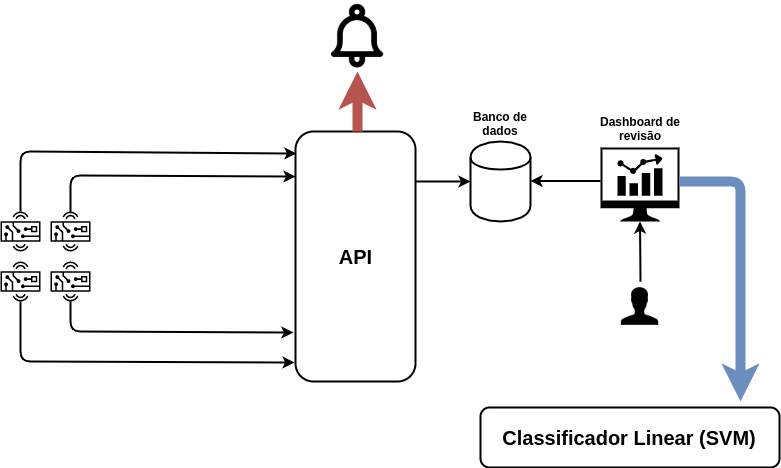
\includegraphics[scale=0.4]{img/fluxoinicial.png}
  \caption{Diagrama esquematizando o fluxo dos dados no início da implementação}
  \label{fig:fluxoinicial}
\end{figure}
  
  \item \textbf{Implementação em pleno funcionamento}: dados suficientes para o treinamento já foram coletados, e existe um modelo de classificador linear disponível para aquele conjunto de câmeras. O fluxo do item anterior continua acontecendo para que o modelo do classificador possa estar em constante evolução, porém a decisão de ativar ou não um alerta é feita com base na decisão do classificador.
  
  \begin{figure}[ht]
  \centering
  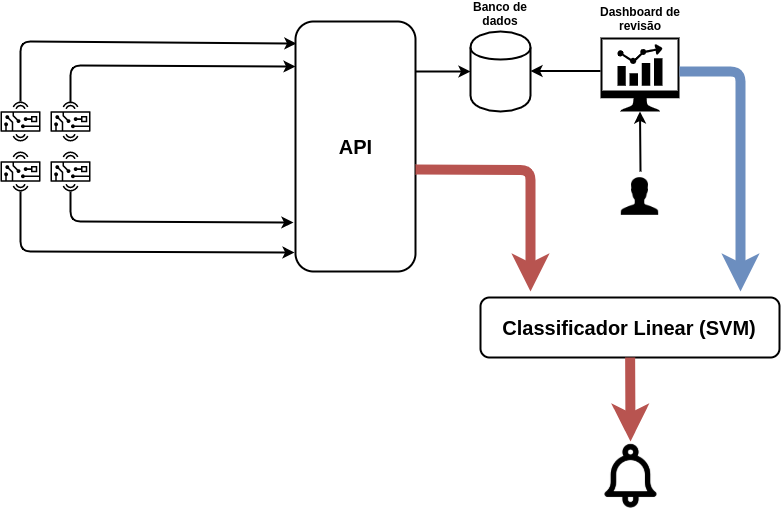
\includegraphics[scale=0.4]{img/fluxofinal.png}
  \caption{Diagrama esquematizando o fluxo dos dados após a implementação completa}
  \label{fig:fluxofinal}
\end{figure}
\end{itemize}

Para tal, foi criada uma API que recebe os dados e os guarda em um banco de dados. Para o caso de uso, o banco de dados escolhido foi MongoDB, devido à sua arquitetura \textit{NoSQL} que permite que não requer que os dados sejam estruturados de maneira fixa, permitindo que o banco esteja adaptável e preparado para futuras mudanças no modelo.

Cada conjunto de câmeras contará com um identificador único chamado de \textit{area\_id}, e cada câmera do conjunto também terá seu identificador único, chamado de \textit{cam\_id}, que, apesar de representar a numeração das câmeras dentro do sistema, também permite que tenhamos controle de câmeras que foram trocadas (e, portanto, reposicionadas ou alteradas). As entradas armazenadas nesse banco de dados contarão com esses dois dados, utilizados para identificar as previsões recebidas, além de um \textit{timestamp}, referente ao horário da ocorrência, e a probabilidade detectada por aquela câmera. Podemos observar a seguir um exemplo de entrada no banco de dados, representativo do \textit{schema} incial que será adotado para a coleta dos mesmos:

\begin{lstlisting}
{'_id': ObjectId('5ded273719c065a57a9512c6'),
 'area_id': '0947f4886c09494490c139ffe2a924b4',
 'cam_id': '896bbb5ad9eb4cf8966afb023a6abca8',
 'dt': datetime.datetime(2019, 12, 8, 13, 39, 19, 841623),
 'prob': 0.7658}
\end{lstlisting}

Optou-se por utiliar identificadores únicos, ou UUIDs, para as áreas em que as câmeras estão localizadas, bem como para as câmeras em si. Com uma probabilidade praticamente nula de colisão, ou seja, de dois identificadores serem o mesmo, os idnetificadores únicos agem aqui como simplificadores. Visto que um dos objetivos da execução em \textit{edge computing} é a diminuição da quantidade de dados trafegada, essa escolha faz com que o \textit{payload} trafegado entre o conjunto de placas e o servidor central seja o mínimo possível, da forma:

\begin{lstlisting}
{'area_id': '0947f4886c09494490c139ffe2a924b4',
 'cam_id': '896bbb5ad9eb4cf8966afb023a6abca8',
 'prob': 0.7658}
 \end{lstlisting}
 
 Totalizando por volta de 160 bytes, um payload dessa forma se torna extremamente atômico, permitindo inclusive que se pense em outras maneiras de se transmitir esse dado que não necessariamente pela internet, visto que a infraestrutura foi planejada para acomodar esse formato de dados.
 
\section{Concepção do classificador linear}

Por fim, definiremos aqui a estrutura do classificador linear a ser utilizado para se criar um \textit{ensemble}. Vale notar, que, seguindo a segmentação dos dados especificadas na seção anterior, existirá um classificador linear para cada área coberta por um conjunto de câmeras, com os parâmetros sendo armazenados e acessíveis pelo servidor central. Para tal, é necessário, para a construção de cada modelo, que ocorrências sejam revistas por operadores humanos.

Para que isso aconteça, deverá haver a coleta periódica das imagens salvas no disco de cada Caninos Loucos. Sob uma análise mais detalhada, e incluindo informações das investigações policiais, as ocorrências serão manualmente marcadas como sendo verdadeiramente, um uso de arma, ou não. As entradas atualizadas no banco de dados passariam a ser do tipo, por exemplo:

\begin{lstlisting}
{'_id': ObjectId('5ded273719c065a57a9512c6'),
 'area_id': '0947f4886c09494490c139ffe2a924b4',
 'cam_id': '896bbb5ad9eb4cf8966afb023a6abca8',
 'dt': datetime.datetime(2019, 12, 8, 13, 39, 19, 841623),
 'prob': 0.7658,
 'is_occurence': True}
\end{lstlisting}

A medida que os dados forem sendo classificados e acumulados, uma rotina assíncrona deverá verificar se existem dados de ocorrência suficientes para o treinamento de um novo modelo. Assim que isso acontecer, todos os dados contidos no banco de dados para um \textit{area\_id} específico serão agregados por períodos de tempo, no caso segundos, e transformados para formato tabular para constituição de um conjunto de dados a ser alimentado à SVM. A tabela \ref{tbl:svmdata} demonstra um exemplo de como essa organização de dados se daria:

\begin{table}[h]
\centering
\begin{tabular}{llllll}
\hline
\multicolumn{1}{|l|}{\textbf{dt}}         & \multicolumn{1}{l|}{\textbf{1}} & \multicolumn{1}{l|}{\textbf{2}} & \multicolumn{1}{l|}{\textbf{3}} & \multicolumn{1}{l|}{\textbf{4}} & \multicolumn{1}{l|}{\textbf{is\_occurence}} \\ \hline
\multicolumn{1}{|l|}{2019-05-04 12:23:20} & \multicolumn{1}{l|}{0.255}      & \multicolumn{1}{l|}{0}          & \multicolumn{1}{l|}{0.365}      & \multicolumn{1}{l|}{0}          & \multicolumn{1}{l|}{1}                      \\ \hline
\multicolumn{1}{|l|}{2019-05-15 15:54:50} & \multicolumn{1}{l|}{0.311}      & \multicolumn{1}{l|}{0.466}      & \multicolumn{1}{l|}{0}          & \multicolumn{1}{l|}{0.543}      & \multicolumn{1}{l|}{0}                      \\ \hline
\multicolumn{1}{|l|}{2019-06-02 13:22:33} & \multicolumn{1}{l|}{0.789}      & \multicolumn{1}{l|}{0.643}      & \multicolumn{1}{l|}{0.622}      & \multicolumn{1}{l|}{0.812}      & \multicolumn{1}{l|}{1}                      \\ \hline
\multicolumn{1}{|l|}{2019-06-02 13:22:34} & \multicolumn{1}{l|}{0.799}      & \multicolumn{1}{l|}{0.702}      & \multicolumn{1}{l|}{0.543}      & \multicolumn{1}{l|}{0.811}      & \multicolumn{1}{l|}{1}                      \\ \hline
                                          &                                 &                                 &                                 &                                 &                                            
\end{tabular}
\caption{Exemplo de dados tabulares a serem alimentados na SVM classificadora}
\label{tbl:svmdata}
\end{table}

Os números 1, 2, 3 e 4 são numerações simplificadas obtidas a partir do número de valores únicos de \textit{cam\_id} para aquele determinado \textit{area\_id}, ou seja, é dependente no número \textit{n} de câmeras. Sendo assim, esse formato tabular tem um número variável de colunas a depender da área de atuação sendo atualizada.

Para o treinamento da SVM, descartamos a coluna \textit{dt} (aqui mostrada apenas para referência), já que para esse modelo, não consideraremos que a hora do dia tem influência sobre a classificação. Sendo assim, nossos parâmetros de entrada para o treinamento serão as colunas referentes às câmeras, e o \textit{output} será a classificação entre 1 ou 0 de \textit{is\_occurence}. A SVM se encarregará de encontrar um hiperplano que, para cada área, separe da melhor maneira as probabilidades coletadas.

Devido à natureza do algoritmo, dos dados e da situação envolvida, não será possível treinar um algoritmo para demonstração: como as probabilidades calculadas são influenciadas por aspectos como posicionamento das câmeras, iluminação e outros fatores externos, é difícil projetar um modelo com dados criados artificialmente, visto que esses não serão capazes de capturar com proximidade o funcionamento desses fatores na vida real. Seria, portanto, necesária a execução de um teste em caráter de prova de conceito para se obter esse resultado. No entanto, a estrutura aqui descrita pode ser aplicada como base para esse processo, sendo compatível com o resto do fluxo descrito. A expectativa é, portanto, que os resultados mostrem uma redução tanto nos falsos negativos quanto nos falsos positivos, e o funcionamento de um sistema que aprende com seus erros, a medida que é corrigido de acordo com a ação humana.

\chapter{Conclusão}

Finalizado todo o processo, conseguimos, a partir da lógica inicial estabelecida e das motivações apresentadas, desenvolver um sistema com funcionamento suficientemente bom que cumpre a proposta delineada. Comprovamos que é possível, de fato, executar algoritmos de inteligência artifical na borda computacional; e mais, algoritmos de detecção de imagem e visão computacional, geralmente associados com hardware mais poderoso e caro.

Baseado nisso, ressalta-se, como demonstrado ao longo deste trabalho, a importância do fator hardware na análise, seja qualitativa ou quantitativa, de algoritmos de inteligência artifical como um todo. Apesar do enfoque ter sido dado à arquitetura de \textit{edge computing}, o princípio vale em qualquer nível de complexidade: é necessário que seja dada a devida atenção ao hardware que baseia as métricas apresentadas, não só para a divulgação de informações mais precisas, mas também para que possamos levar esses algoritmos aos seus limites, procurando ampliar seu uso e efetividade.

Prova disso é a simplificação dos modelos YOLO realizada neste trabalho, que fez com que um algoritmo de detecção de imagem referência, porém que exige GPUs avançadas para execução, conseguisse ser executado em uma placa comparativamente muito mais simples e miniaturizada. Descobertas como essa reforçam o \textit{edge computing} como paradigma dominante nas práticas de Internet das Coisas no futuro, permitindo que tarefas sejam feitas mais rapidamente, de maneira local e, principalmente, consumindo pouca energia e desonerando a largura de banda da internet. Isso faz com que possamos avançar tecnologicamente de maneira extremamente rápida, sem depender de fatores externos como a vinda de uma nova tecnologia, como o 5G.

Destaca-se, nesse cenário, a placa Caninos Loucos. Tanto seu hardware foi capaz de dar conta da tarefa em questão, postas as limitações, quanto sua arquitetura aberta conforma com questões ainda um pouco negligenciadas no campo de tecnologia, porém extremamente relevantes na sociedade e principalmente no uso da tecnologia em conjunto com instituições pública, como transparência e governança. Como um hardware ainda em desenvolvimento e evolução, espera-se que este seja apenas um ponto de início.

Não podemos ignorar, no entanto, as concessões feitas para que todas as conquistas anteriormente mencionadas pudessem ser antingidas. Fica claro, assim, a relação inversamente proporcional entre velocidade e eficiência. As limitações do hardware nos impuseram perdas na precisão dos modelos e na velocidade. Apesar de termos conseguido um tempo de resposta extremamente satisfatório, vale reforçar a seriedade de classificações erradas no caso de uso presente, onde a vida de seres humanos pode estar em risco. A chave, então, reside em equilibrar essa relação.

A abordagem multicâmera, portanto, representa uma solução inovadora nesse campo, fazendo com que as desvantagens encontradas pelo caminho sejam recombinadas para um fortalecimento mútuo. Apesar de representar um pequeno distanciamento da arquitetura de \textit{edge computing} ideal, essa abordagem representa uma solução suficientemente eficaz e barata para o problema, dadas as condições atuais.

É notável que a solução aqui apresentada ainda apresenta muito espaço para evolução. Apesar da taxa de precisão do algoritmo treinado atingir bons patamares, inclusive superando alguns modelos de referência, sempre é possível otimizá-lo, sendo pela proposição de diferentes modelos simplificados (talvez baseados em versões mais recentes), adaptações no conjunto de treino (podendo ser utilizadas imagens coletadas pelas próprias câmeras durante ocorrências reais) ou até um período de treinamento mais longo (sempre tomando cuidado para evitar o sobreajuste).

Paralelamente, como mencionado, também é esperada uma evolução na plataforma Caninos Loucos, que prevê a implementação de uma GPU em sua estrutura em breve. Essa evolução terá grandes impactos sobre os resultados desse trabalho, abrindo um leque de possibilidades para seu aperfeiçoamento. Dada a relação entre performance e eficiência já apresentada, poderá se escolher entre um algoritmo mais rápido, que poderá realmente se aproximar do \textit{real-time}, mantendo a precisão; um algoritmo mais preciso, no entanto, na velocidade atual; ou uma mistura de ambas as coisas, a depender do caso de uso. Ressalta-se, no entanto, a necessidade do ecossistema de inteligência artificial de ampliar seus horizontes para além do ambiente proprietário CUDA, da NVIDIA, em torno do qual todas as ferramentas mais conhecidas giram em torno atualmente. Seguindo a ideia de uma arquitetura aberta e transparente, é necessário que esses princípios sejam mantidos no âmbito do aprendizado de máquina.

Da mesma forma, essas melhorias, consequentemente, serão responsáveis por fazer com que seja repensada a função da topologia multicâmera nessa aplicação. Inicialmente concebida como uma forma de compensação das concessões feitas em decorrência do hardware, uma vez que essas concessões deixam de existir, a infraestrutura pode ser aproveitada para outros benefícios: desde uma precisão ainda maior, até um monitoramento mais complexo. Além disso, uma vez que introduzimos agentes humanos no \textit{loop} algorítmico, é importante que essa relação seja sempre observada e revisada. A interferência humana é benéfica ou prejudicial ao funcionamento do meu sistema? Obras como \citeyear{wmd} \citeauthor{wmd} apontam consequências desastrosas causadas por descuidos da ação humana sobre algoritmos. No nosso caso, no entanto, a única forma de se atingir o objetivo proposto é se valendo dessa ação. Essa interação deve sempre ser equilibrada.

Encerra-se, portanto, esse ciclo de trabalho com uma solução prática em mãos, na esperança de que ela possa servir de maneira positiva e justa à sociedade, e que seu desenvolvimento e melhorias sejam constantes, representando evoluções tecnológicas e científicas que sempre avancem na direção dos princípios e motivações aqui estabelecidos.

% ========== Referências ==========
% --- IEEE ---
%	http://www.ctan.org/tex-archive/macros/latex/contrib/IEEEtran
%\bibliographystyle{IEEEbib}

% --- ABNT (requer ABNTeX 2) ---
%	http://www.ctan.org/tex-archive/macros/latex/contrib/abntex2
\bibliographystyle{abntex2-num}

\bibliography{referencias.bib}

\apendice{}
\chapter{Definição das métricas de performance do modelo}

Apresentamos, nesse apêndice, de forma rápida, as definições matemáticas das métricas de performance dos modelos de aprendizado de máquina referidos ao longo do trabalho.

\begin{itemize}
    \item \textbf{P}: Precisão
    \begin{equation}
        P = \frac{Positivos\; Verdadeiros}{Positivos\; Verdadeiros + Falsos\; Positivos}
    \end{equation}
    
    \item \textbf{R}: Recall
    \begin{equation}
        R = \frac{Positivos\; Verdadeiros}{Positivos\; Verdadeiros + Falsos\; Negativos}
    \end{equation}
    
    \item \textbf{AP}: \textit{Average Precision} ou Precisão Média
    
    Onde \textit{p(r)} é uma curva de precisão em função de recall, ordenadas de maneira decrescente pelas probabilidades retornadas pelo modelo, para cada classe:
    
    \begin{equation}
        AP = \int_{0}^{1}p(r)dr
    \end{equation}
    
    \item \textbf{mAP}: \textit{Mean Average Precision} ou Média das Precisões Médias
    
    Onde \textit{K} é o número total de classes:
    
    \begin{equation}
        mAP = \frac{\sum_{k=1}^{K} AP(k)}{K}
    \end{equation}
    
    \item \textbf{F1}: F1-score
    
    \begin{equation}
        F1 = 2 \times \frac{F \times P}{F + P}
    \end{equation}
    
    \item \textbf{IoU}: \textit{Intersection over Union} (Intersecção sobre União)
    
    Onde I é a intersecção entre a \textit{bounding box} predita e a \textit{bounding box} real, e U é a união de ambas as duas \textit{bounding boxes}, em uma única observação:
    
    \begin{equation}
    IoU = \frac{I}{U}
    \end{equation}
    
    \item \textbf{mIoU}: IoU médio
    
    Onde Q é o número total de observações:
    
    \begin{equation}
        mIoU = \frac{\sum_{q=1}^{Q} IoU(q)}{Q}
    \end{equation}
    
\end{itemize}

\chapter{Disponbilização do modelo e código-fonte}

Seguindo as práticas especificadas no primeiro capítulo do trabalho, todo o código utilizado no desenvolvimento do algoritmo, bem como os pesos referentes ao modelo pronto serão disponibilizados online sob uma licença MIT. Sendo assim, optou-se por fazer essa distribuição por meio de um repositório no GitHub. O conteúdo pode ser encontrado em:

\center\url{https://github.com/felipecgonc/moirai}

\end{document}
